\documentclass[xcolor=dvipsnames]{beamer}

\usetheme{Darmstadt}
\usefonttheme[onlylarge]{structurebold}
\setbeamerfont*{frametitle}{size=\normalsize,series=\bfseries}
\setbeamertemplate{navigation symbols}{}

\usepackage[english]{babel}
\usepackage[cp1250]{inputenc}
\usepackage{times}
\usepackage[T1]{fontenc}


\usepackage{graphicx,amsmath} % Add all your packages here
\usepackage{amsfonts}
%\usepackage{listings}


\usepackage{url}

\usepackage{tikz}
\usetikzlibrary{arrows}
\tikzstyle{block}=[draw opacity=0.7,line width=1.4cm]


% correct bad hyphenation here
\hyphenation{op-tical net-works semi-conduc-tor IEEEtran}


\title{Web Information Extraction Systems\\for Web Semantization}

\author[D�dek]
{Jan D�dek\inst{1,2}}

\institute[MFF UK and CS CAS]
{
  \inst{1}%
Department of Software Engineering, Faculty of Mathematics and Physics, Charles University in Prague, Czech Republic
  \and
  \inst{2}%
Institute of Computer Science, Academy of Sciences of the Czech Republic
}

\date[SAIAW WI 2009]
{ITAT 2009\\28 September, Kralova studna}



\begin{document}

\begin{frame}
  \titlepage
\end{frame}

\begin{frame}{Outline}
  \tableofcontents
\end{frame}


\section{Introduction} 
\subsection{The Semantic Web in Use}


\begin{frame}{The Semantic/Semantized Web in Use}
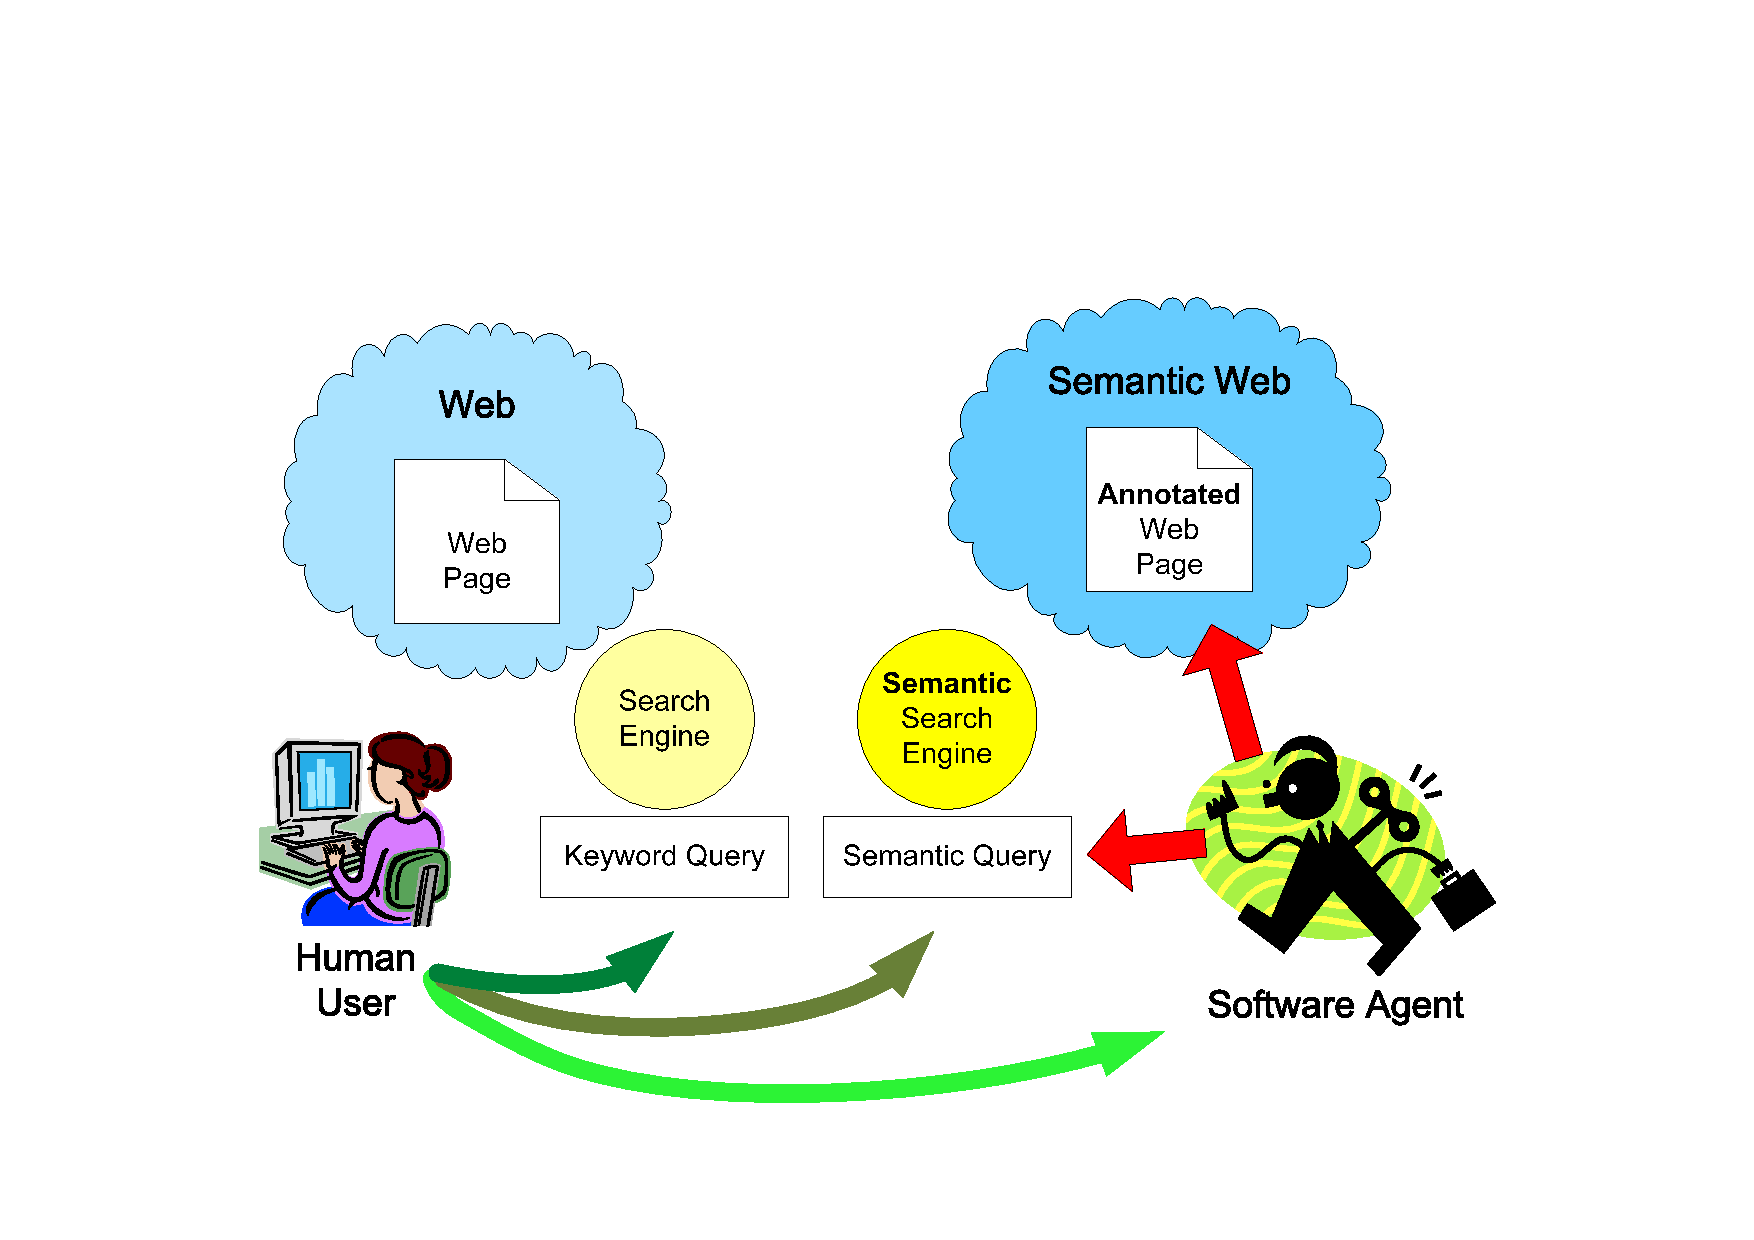
\includegraphics[width=\hsize]{img/SemanticWeb}
\end{frame}

\begin{frame}{Growing of Linking Open Data data set 2007--2008}
\framebox{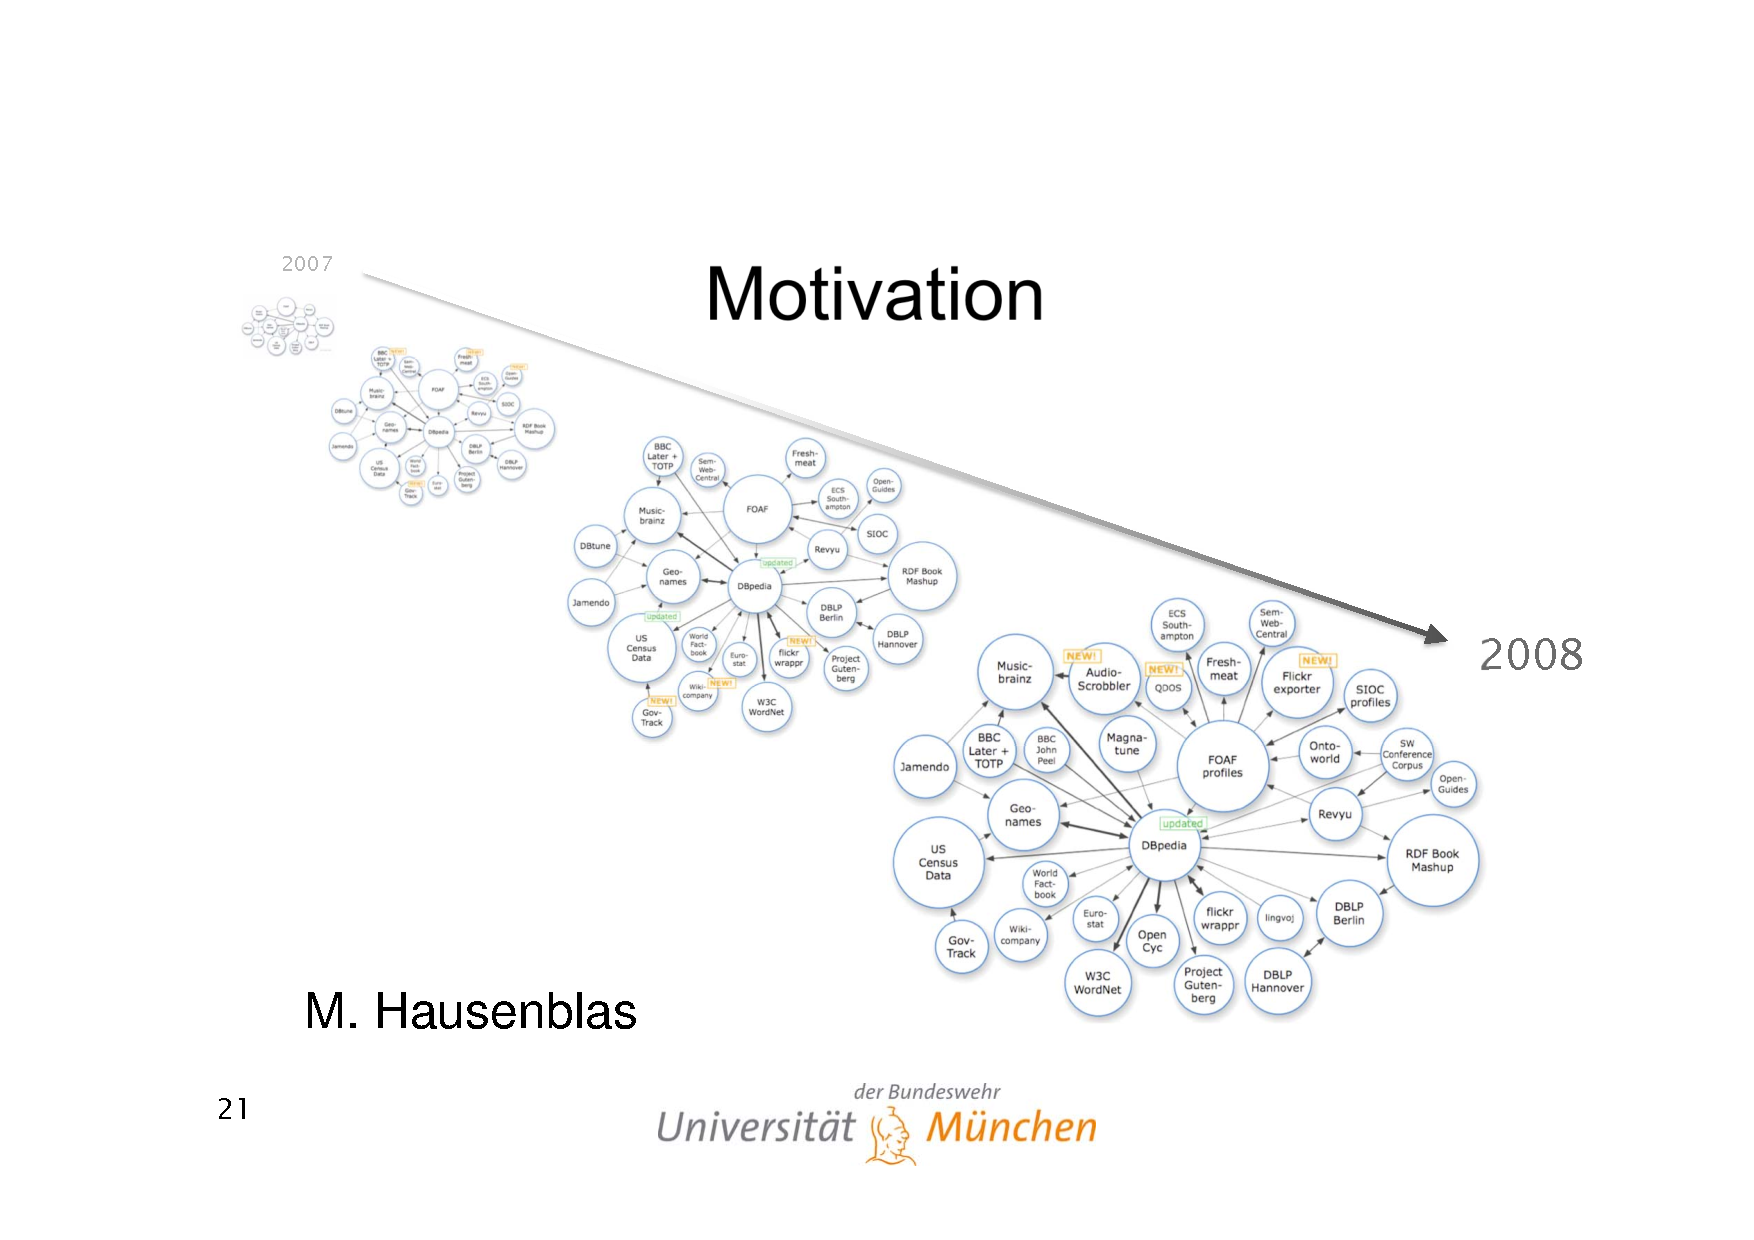
\includegraphics[width=\hsize]{img/LOD2007}}
\end{frame}

\begin{frame}{Growing of LOD data set 2008--2009}
\framebox{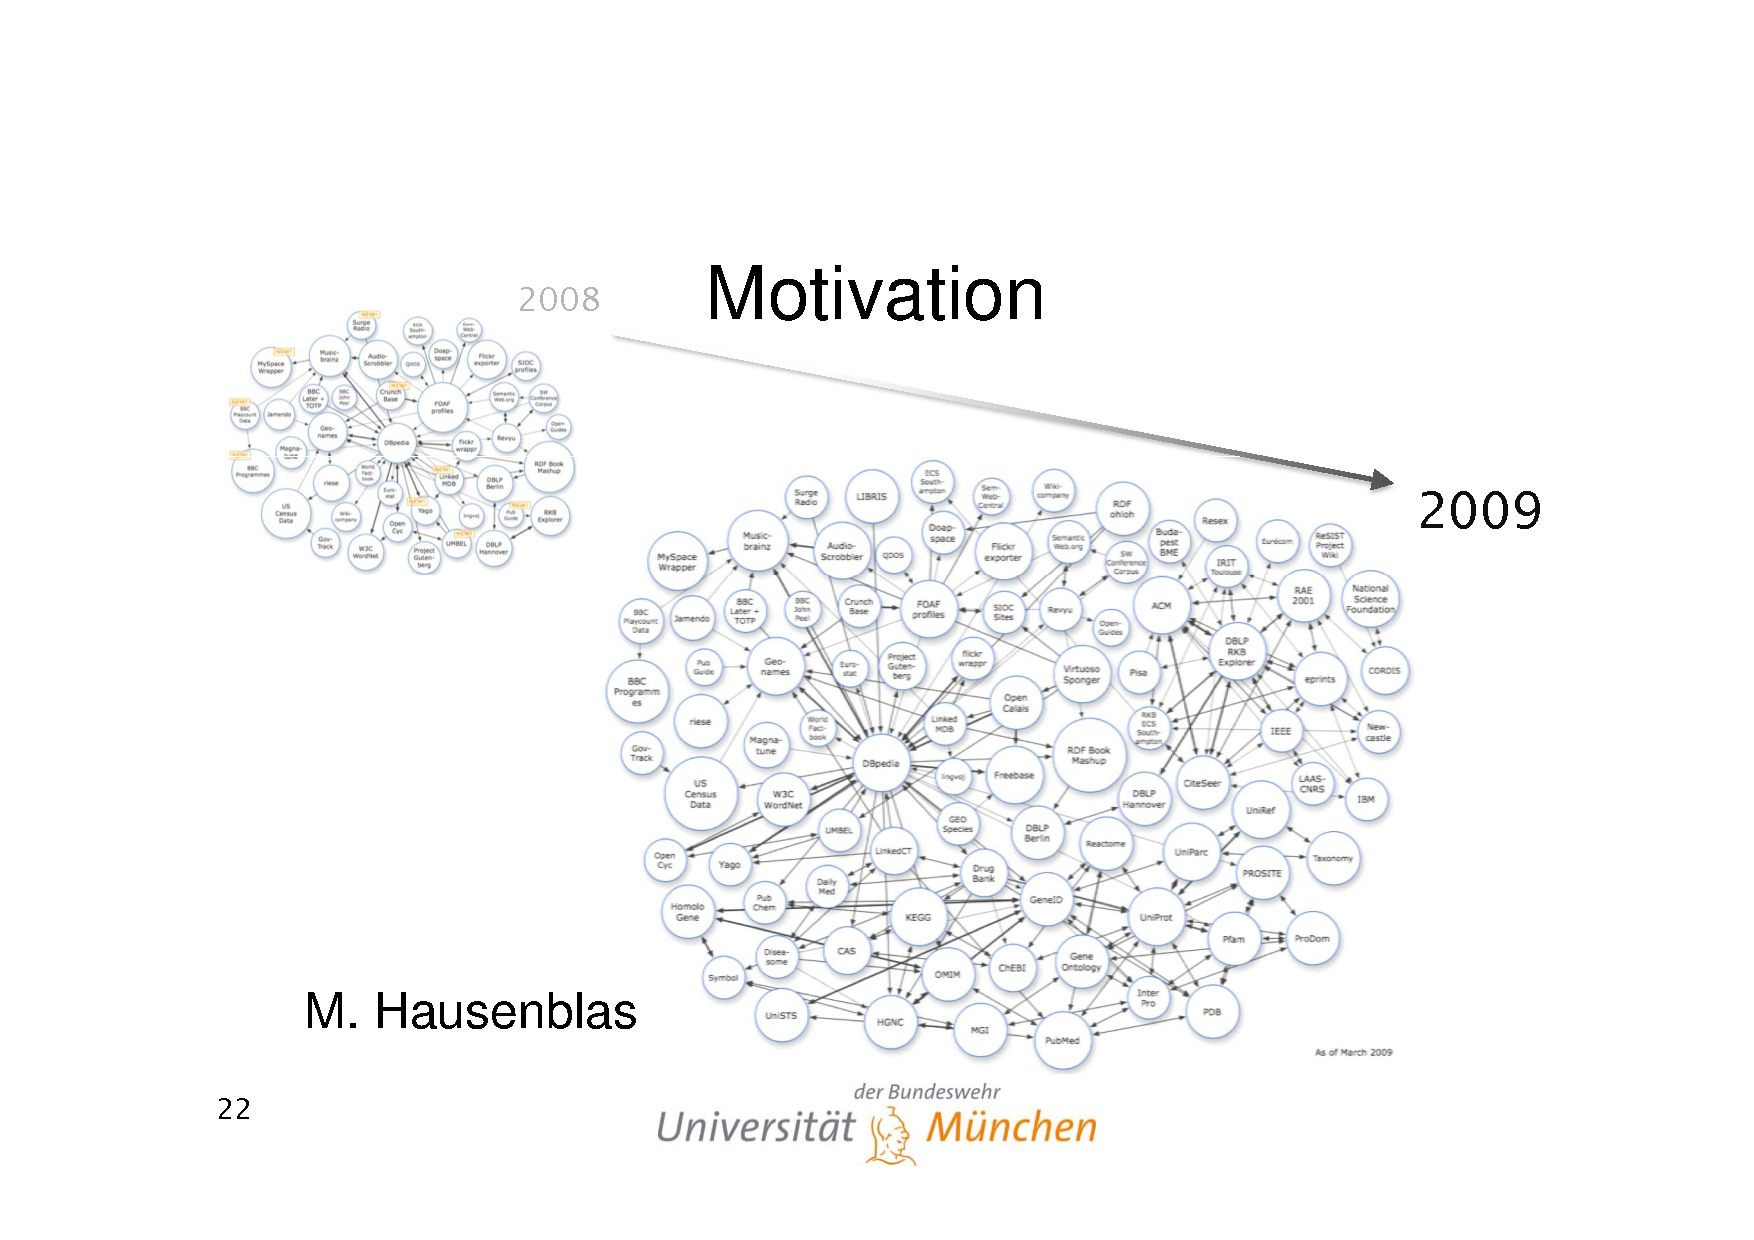
\includegraphics[width=\hsize]{img/LOD2008}}
\end{frame}

\begin{frame}{LOD data set statistics as of July 2009}

\includegraphics[width=0.5\hsize]{img/LoDLogo}
\bigskip\\
\centerline{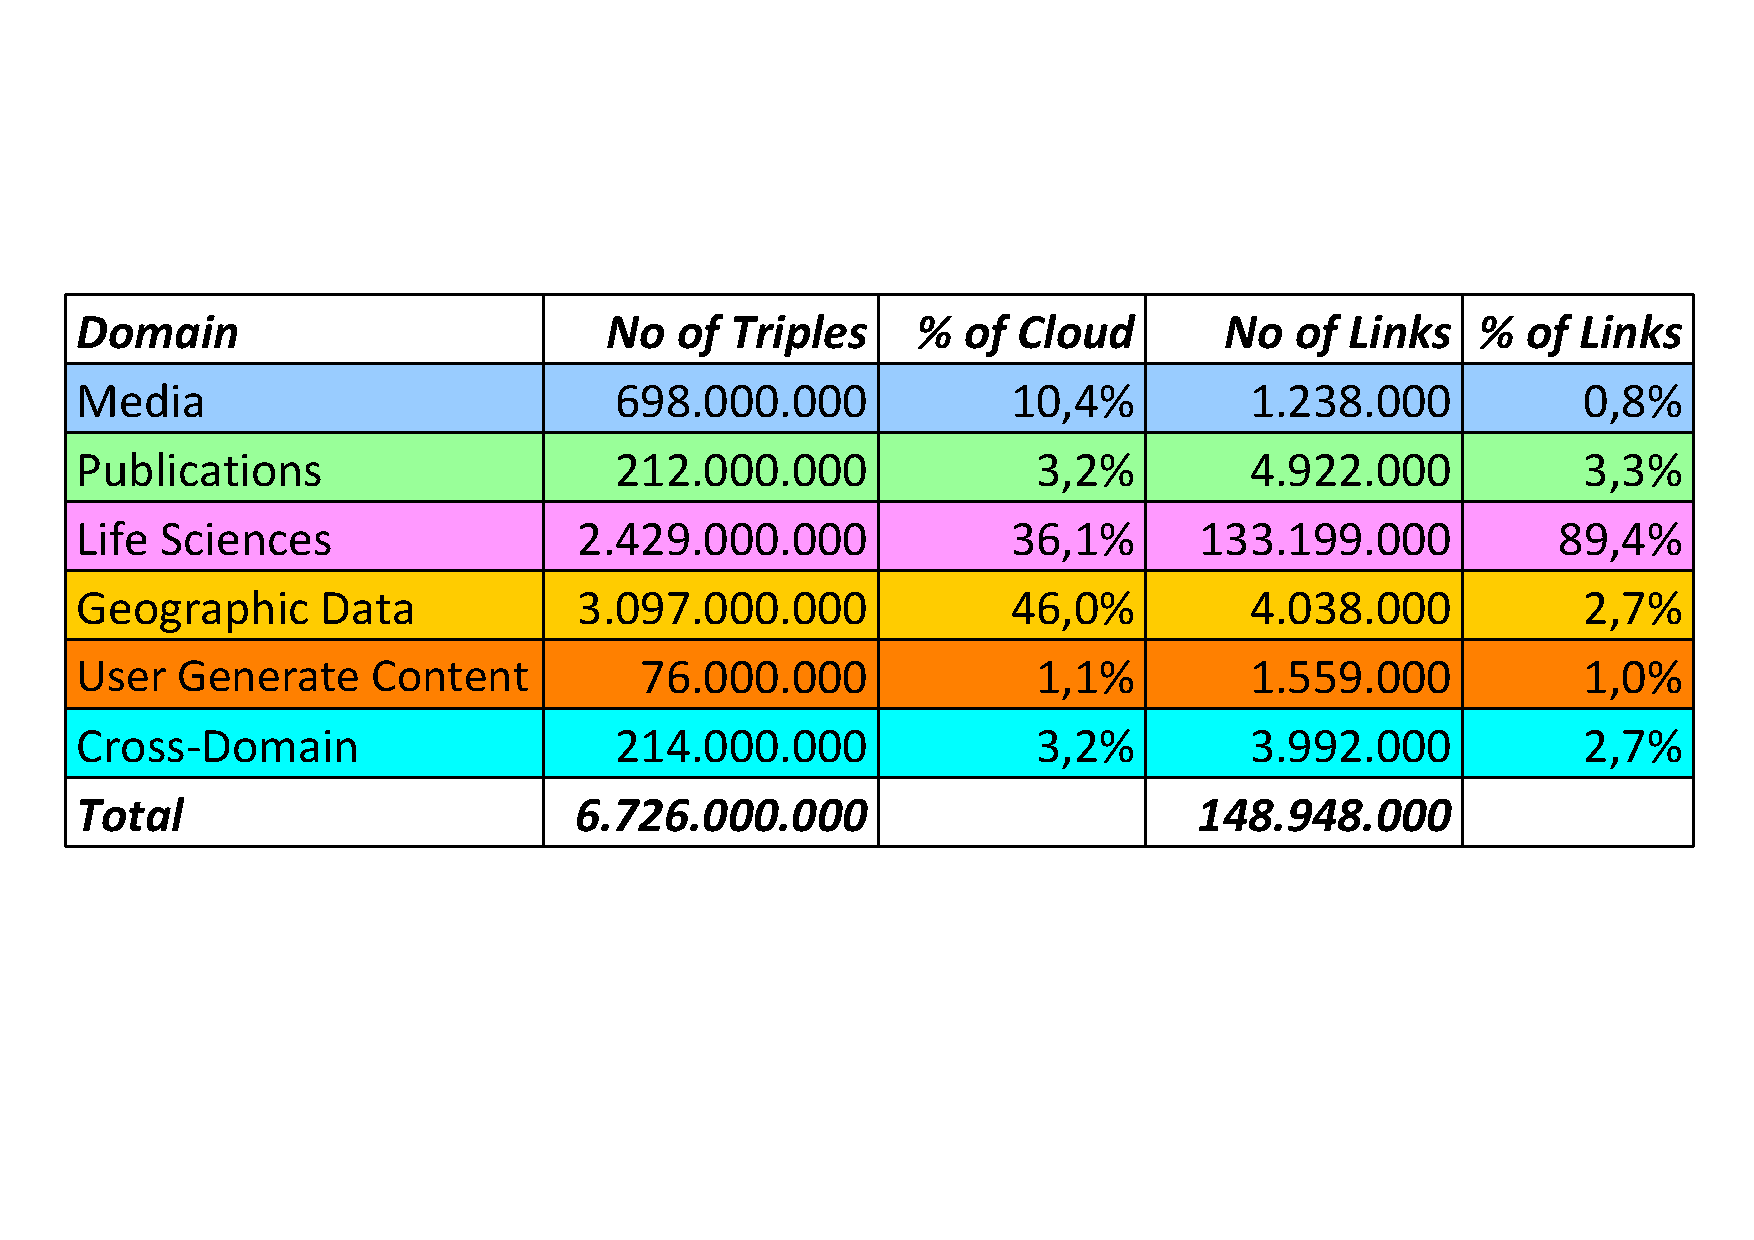
\includegraphics[width=\hsize]{img/Chris}}
\medskip
Christian Bizer: The Web of Linked Data (26/07/2009)
\end{frame}


\begin{frame}[plain]
\centerline{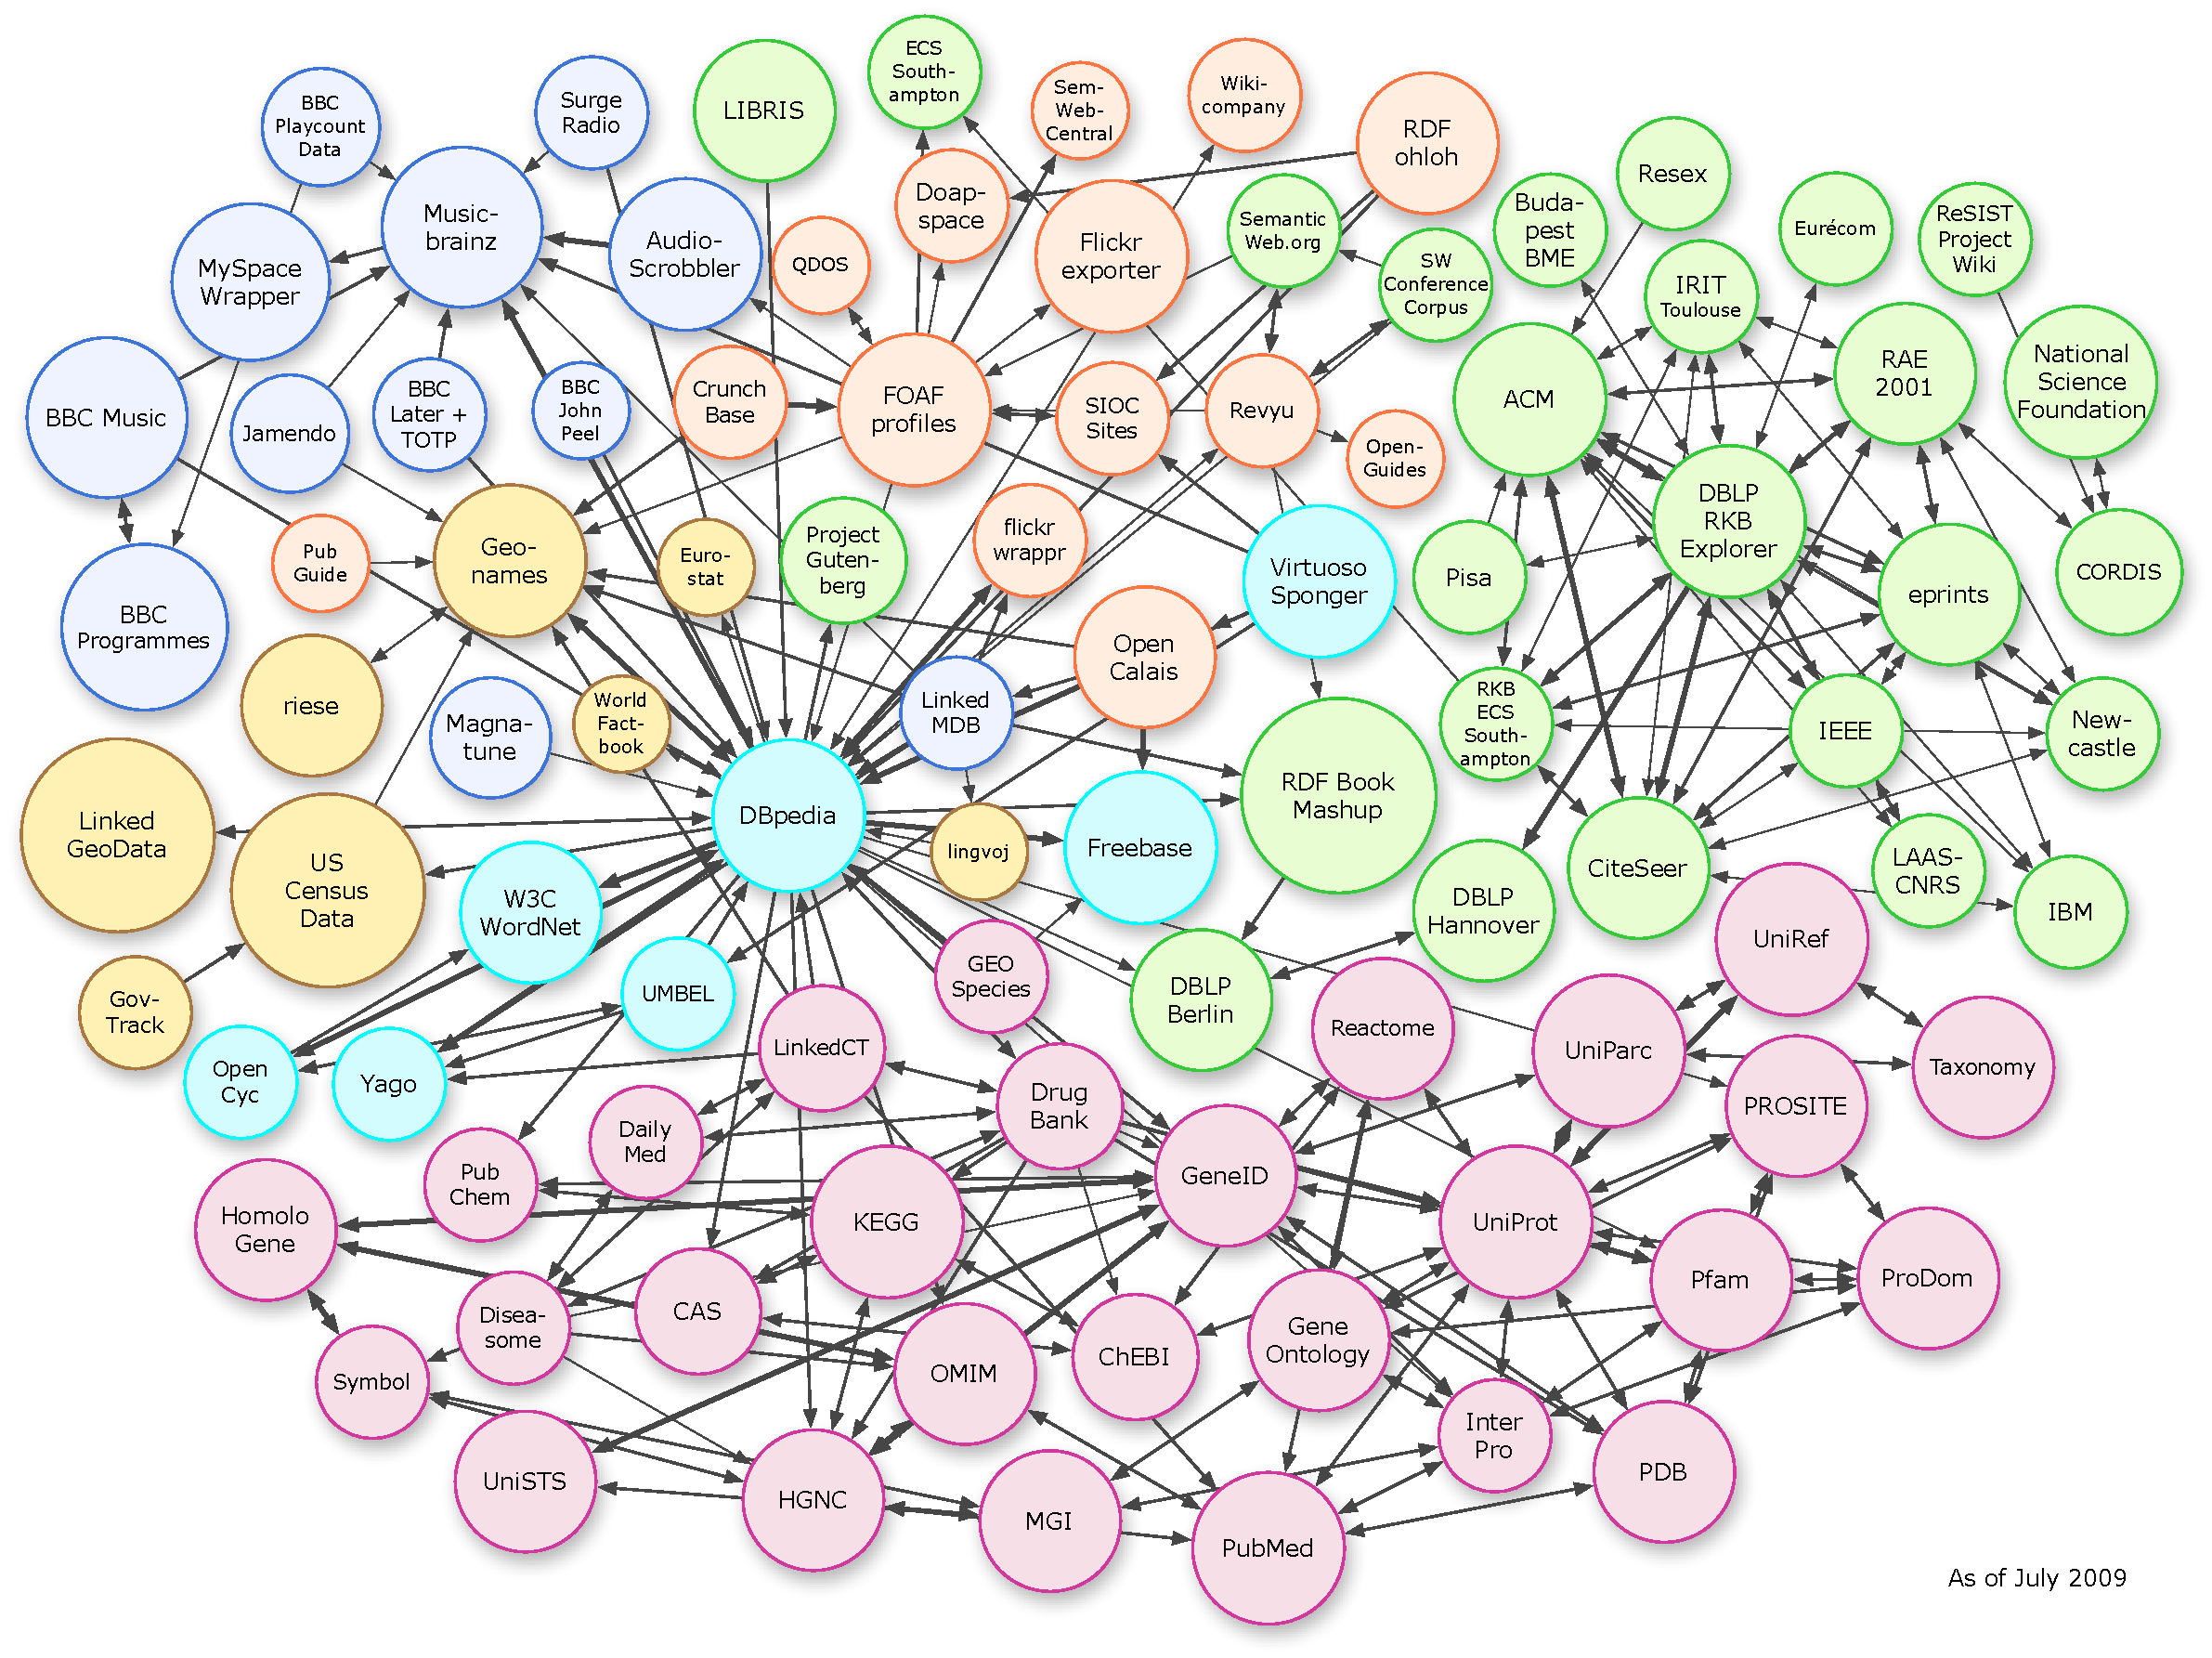
\includegraphics[width=1.19\hsize]{img/lod-datasets_2009-07-14_colored}}
\end{frame}

\subsection{Web Semantization}

\begin{frame}{Web Semantization}
\centerline{\includegraphics[height=0.9\vsize, width=0.7\hsize]{img/semantization}}
\end{frame}

\section{Web Information Extraction}

\subsection{Web Information Extraction Approaches}

\begin{frame}{Division of extraction methods}
\centerline{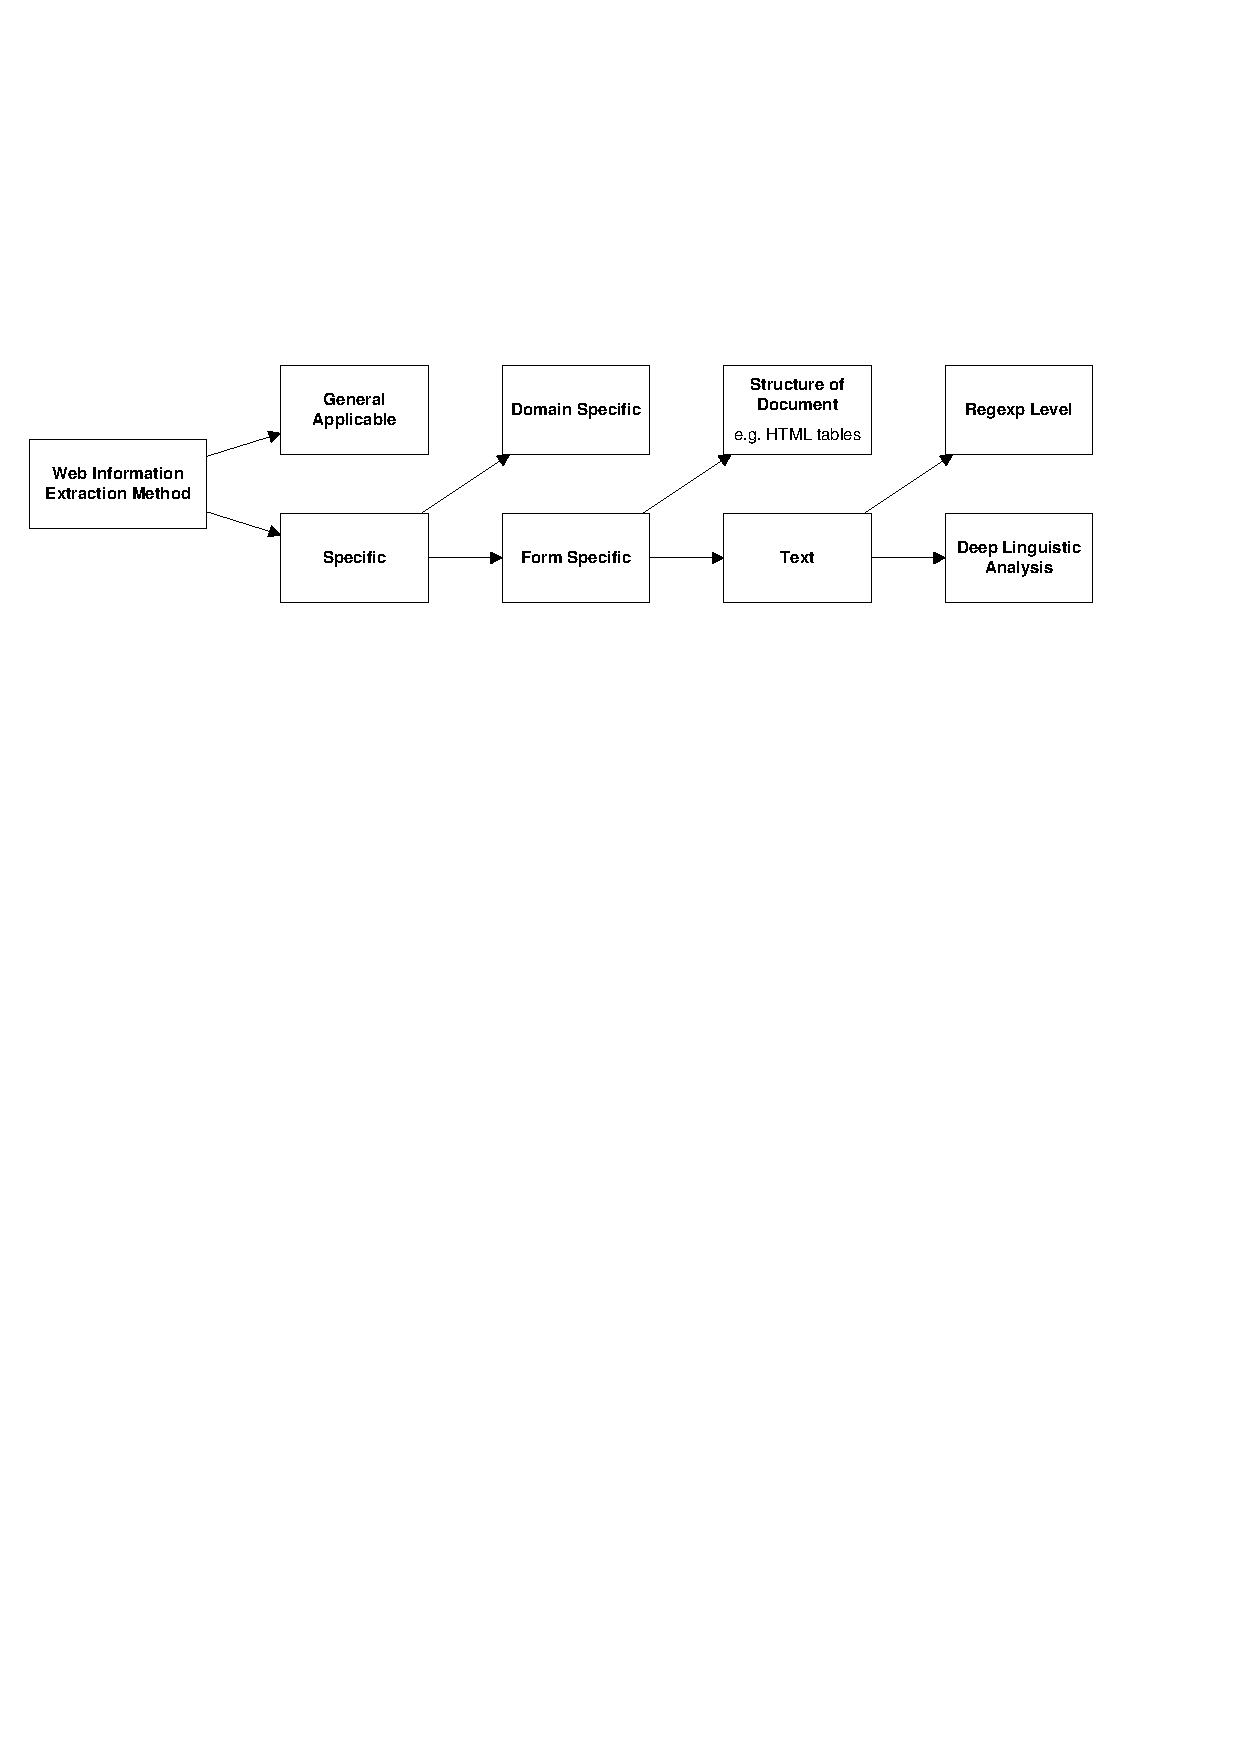
\includegraphics[width=1.15\hsize]{img/extraction_method}}
\begin{itemize}
\item{General Applicable}
\begin{itemize}
	\item \alert{Instance Resolution Task}
\begin{itemize}
	\item 	Bootstraping
	\item 	Use of search engines
\end{itemize}
\end{itemize}
\item{Domain Specific}
\item{Form Specific}
\end{itemize}
\end{frame}


\subsection{User Initiative and Effort}


\begin{frame}{A general view of WI systems -- user perspective}
\centerline{\includegraphics[width=\hsize]{img/WIE_survey}}
\end{frame}


\begin{frame}{User initiative and effort -- Web Semantization}
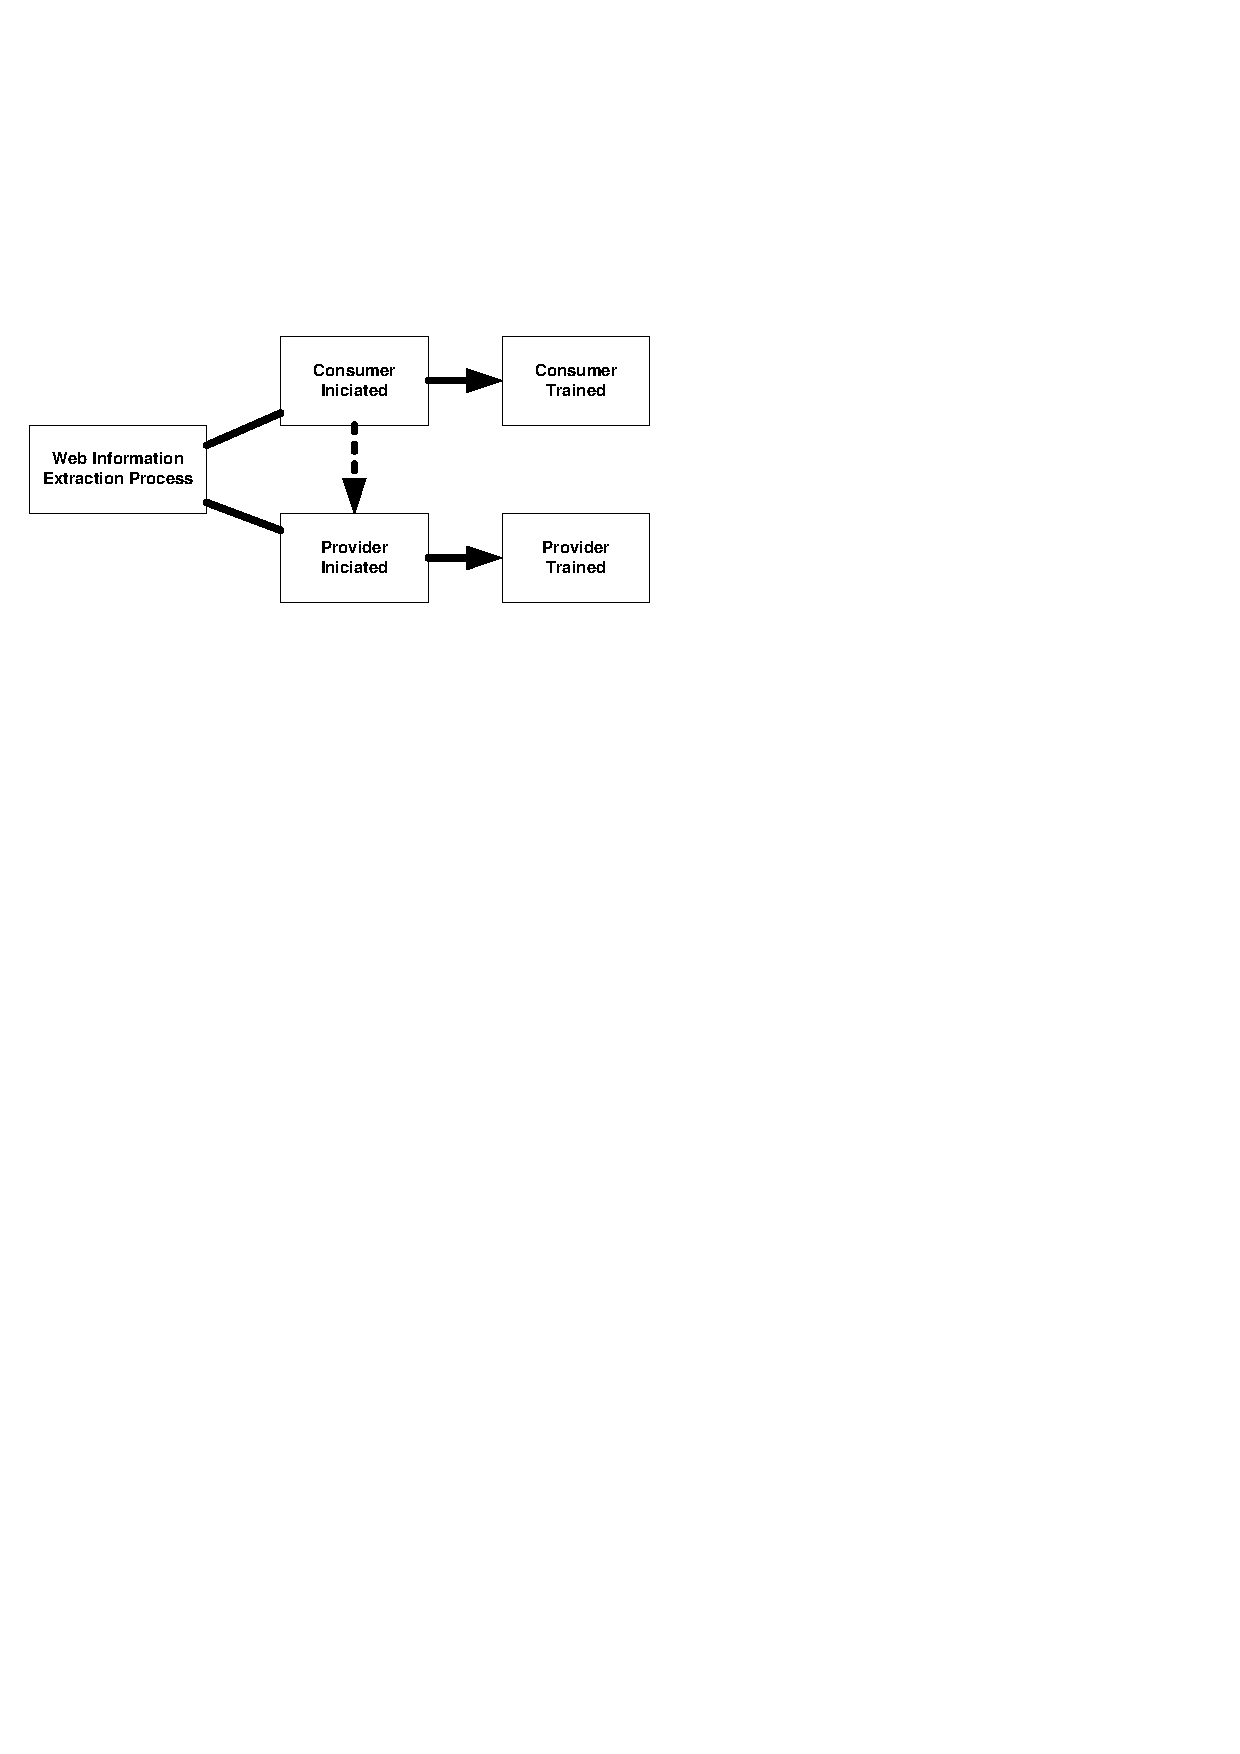
\includegraphics[width=\hsize]{img/extraction_proces_and_user}
\begin{itemize}
	\item Not only Information Extraction
	\item But also Semantic Annotation
	\item Domain specific knowledge has to be \alert{obtained} in all cases.
	\item Scalability?
\end{itemize}
\end{frame}




%\subsection{Alternative Solutions}

%wikipedia

%hodnoceni - tez velmi relevantni k semantickemu webu

\subsection{Information Extraction based on Web Page Structure}
\begin{frame}{Extraction Based on Structural Similarity (suitable for Web Shops)}
\includegraphics[width=\hsize]{img/maruscak}
\end{frame}

\begin{frame}{Extraction Based on Structural Similarity -- extraction method}
\centerline{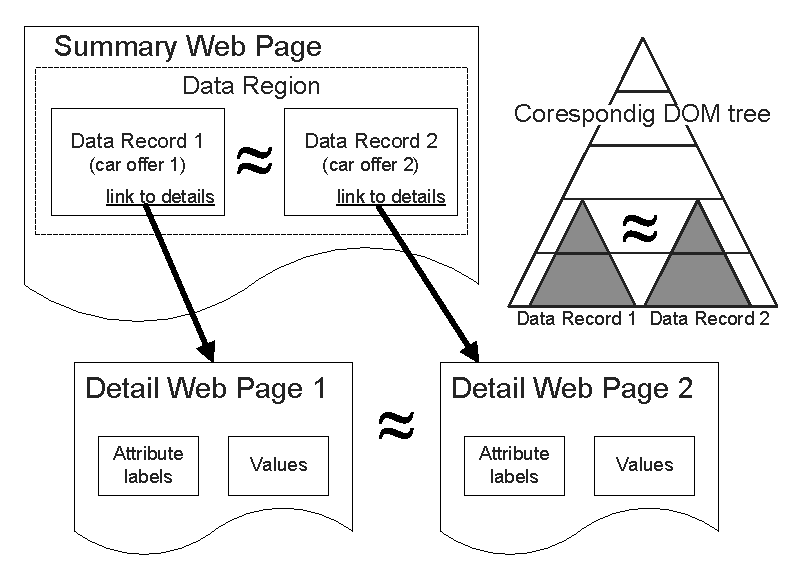
\includegraphics[width=0.8\hsize]{img/StructuralSimilarity}}
\end{frame}


\subsection{Information Extraction from Text-based Resources}

%\subsection{Tasks of Information Extraction}

\begin{frame}{Benchmarks for Information Extraction}
\begin{itemize}
	\item No common benchmark for \alert{``structured pages'' or Web IE}.
	\bigskip
	\item Message Understanding Conference (MUC)
	\item Automatic Content Extraction (ACE) Evaluation
	\item Text Analysis Conference (TAC)
	\medskip
	\item Text REtrieval Conference (TREC)
	\item Document Understanding Conferences\\(text summarization)
\end{itemize}
\end{frame}


\begin{frame}{Classical tasks of text preprocessing and linguistic analysis}
\begin{description}
	\item[Text Extraction] -- e.g from HTML, PDF or DOC,
	\item[Tokenization] -- detection of words, spaces, punctuations, etc.,
	\item[Segmentation] -- sentence and paragraph detection,
	\item[POS Tagging] -- part of speech assignment, often including lemmatization and morphological analysis,
	\item[Syntactic Analysis] (often called linguistic \emph{parsing}) -- assignment of the grammatical structure to given sentence with respect to given linguistic formalism (e.g. formal grammar),
	\item[Coreference Resolution] (or \emph{anaphora resolution}) -- resolving what a pronoun, or a noun phrase refers to. These references often cross boundaries of a single sentence.
\end{description}
\end{frame}

\begin{frame}{Classical domain dependent IE tasks}
\begin{description}
	\item[Named Entity Recognition:] This task recognizes and classifies named entities such as \alert{persons, locations, time expression, or measuring units}. %More complex patterns may also be recognized as structured entities such as addresses.
	\item[Template Element Construction:] Populates templates describing entities with extracted
\alert{roles} (or \alert{attributes}) about one single entity. %This task is often performed stepwise sentence by sentence, which results in a huge set of partially filled templates.
	\item[Template Relation Construction:] As each template describes information about one single entity, this tasks identifies semantic \alert{relations between entities}.
	\item[Template Unification:] \alert{Merges} multiple elementary templates filled with \alert{information about identical entities}.
	\item[Scenario Template Production:] Fits Template Elements and Template Relations into templates describing pre-specified event scenarios (\alert{pre-specified ``queries on the extracted data''}).
\end{description}
\end{frame}


\begin{frame}{Linguistic IE and Semantic interpretation of extraction rules}
\centerline{\includegraphics[width=1.16\hsize]{img/DedVoj_semantic_interpretation}}
\begin{itemize}
	\item Determines how particular values of attributes are used.
	\item Gives semantics to extraction rule.
	\item Gives semantics to extracted data.
\end{itemize}
\end{frame}

\begin{frame}{Linguistic IE -- ILP Learning of Extraction Rules}
\includegraphics[width=0.95\hsize]{img/ILP_learning}
\end{frame}


\section{Conclusion and Future Work}

\begin{frame}{Conclusion and Future Work}
Conclusion:
\begin{itemize}
	\item Partial survey of WIE systems\\(see the paper for references)
	\begin{itemize}
		\item Related to \alert{Web Semantization}
	\end{itemize}
	\item Problem of \alert{unskilled user} pointed out
\end{itemize}
	\vspace{1cm}
Future Work:
\begin{itemize}
	\item Future \alert{development of WIE} tools and work on their adaptability to new domains.
	\item \alert{Integration} of WIE tools to the web semantization system.
	\item Development of the methodology and software to support the \alert{extension} of the semantization system \alert{to a new domain for a non-expert user}.
\end{itemize}
\end{frame}


\end{document}





%
%
%\subsection{Our Information Extraction System}
%
%\begin{frame}{Our work}
%\begin{itemize}
%	\item Extraction of semantic information form \alert{texts}.	
%		\begin{itemize}
%			\item In Czech language.
%			\item Coming form web pages.
%		\end{itemize}
%	\item Using of Semantic Web \alert{ontologies}.
%		\begin{itemize}
%			\item RDF, OWL
%		\end{itemize}
%	\item Exploiting of linguistic tools.
%		\begin{itemize}
%			\item Mainly from the \alert{Prague Dependency Treebank} project.
%			\item Experiments with the Czech WordNet.
%		\end{itemize}
%	\item \alert{Rule based} extraction method.
%		\begin{itemize}
%			\item Extraction rules $\approx$ \alert{tree queries}
%			\item ILP learning of extraction rules
%		\end{itemize}
%	\bigskip
%	\item Fuzzy report classification
%		\begin{itemize}
%			\item Application of \alert{Fuzzy ILP}
%			\item Accident seriousness classification
%			\item Exploitation of extracted information
%		\end{itemize}
%\end{itemize}
%\end{frame}
%
%
%\begin{frame}{Schema of the whole system}
%\begin{columns}
%\column{.45\textwidth}
%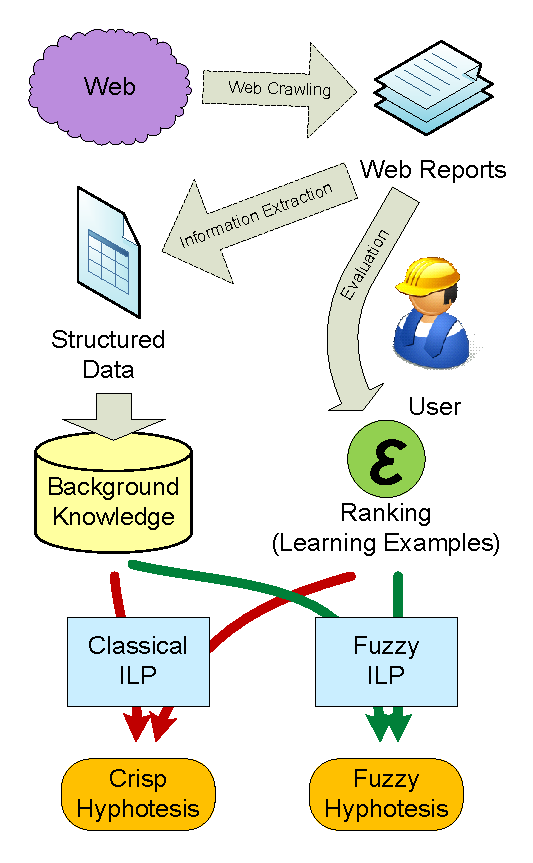
\includegraphics[height=0.9\vsize]{img/schema}
%\column{.55\textwidth}
%\begin{enumerate}
%	\item Web Crawling
%	\item Information Extraction and User Evaluation
%	\item Logic representation
%		\begin{itemize}
%			\item Construction of \alert{background knowledge}
%			\item Construction of \alert{learning examples}
%		\end{itemize}
%	\item ILP Learning
%		\begin{itemize}
%			\item Crisp
%			\item Fuzzy
%		\end{itemize}
%		
%	\bigskip
%	\item Comparison of results
%\end{enumerate}
%
%\end{columns}
%\end{frame}
%
%
%
%\begin{frame}{Example of processed web page}
%\begin{columns}
%\column{.6\textwidth}
%\includegraphics[height=0.9\vsize]{img/DedVoj_article}
%\column{.4\textwidth}
%\begin{itemize}
%	\item Fire and car accidents reports
%\end{itemize}
%\end{columns}
%\end{frame}
%
%\begin{frame}{Example of processed text}
%\centerline{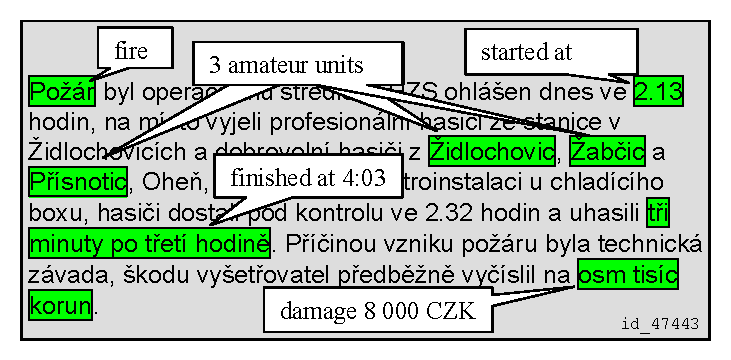
\includegraphics[height=0.5\vsize]{img/message}}
%\bigskip
%\begin{itemize}
%	\item Information to be extracted is decorated.
%	\item See the last sentence on the \alert{next slide}.
%\end{itemize}
%\end{frame}
%
%\begin{frame}{Example of a linguistic tree}
%\centerline{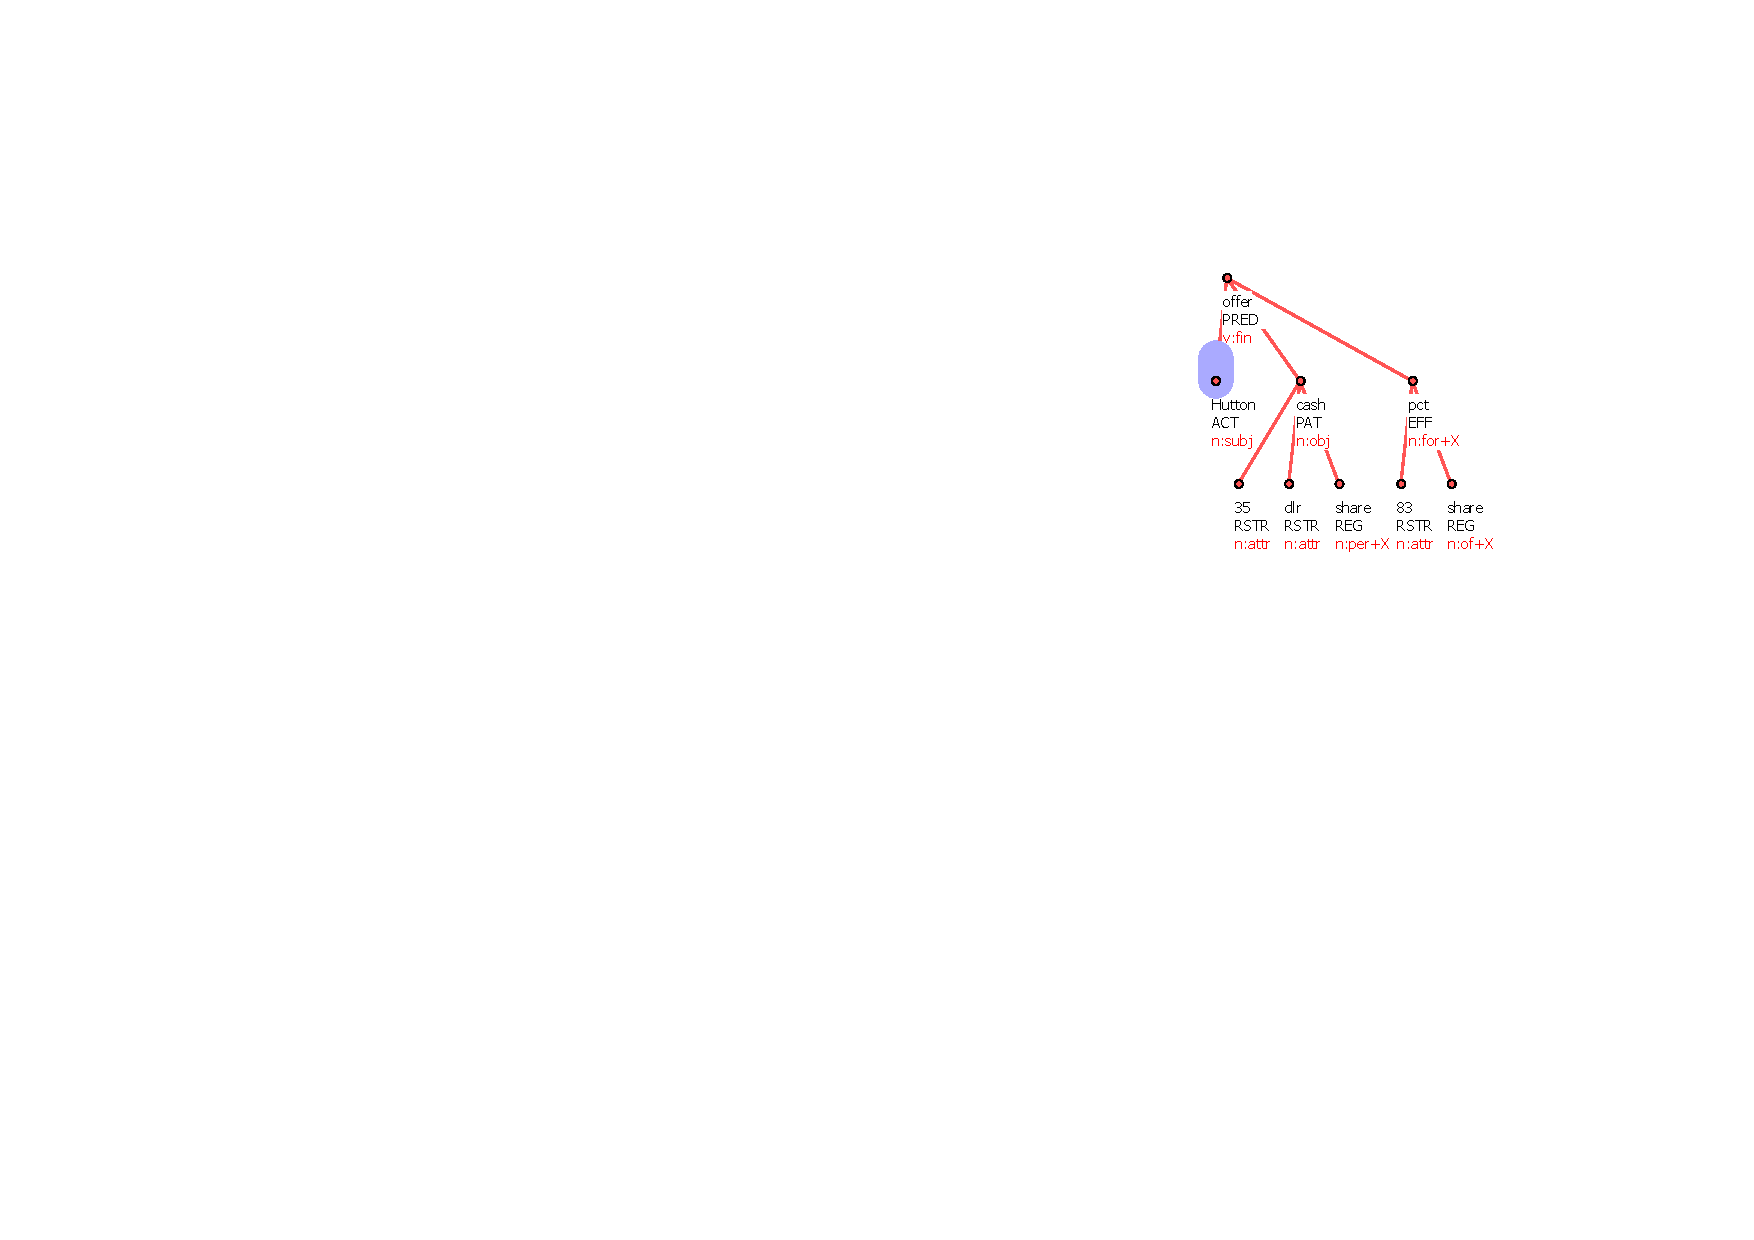
\includegraphics[height=0.7\vsize]{img/tree}}
%\begin{itemize}
%	\item Our IE method uses \alert{tree queries} (tree patterns)
%\end{itemize}
%\end{frame}
%
%
%\subsection{Description of the extraction method}
%
%\begin{frame}{Extraction rules -- Netgraph queries}
%\begin{center}
%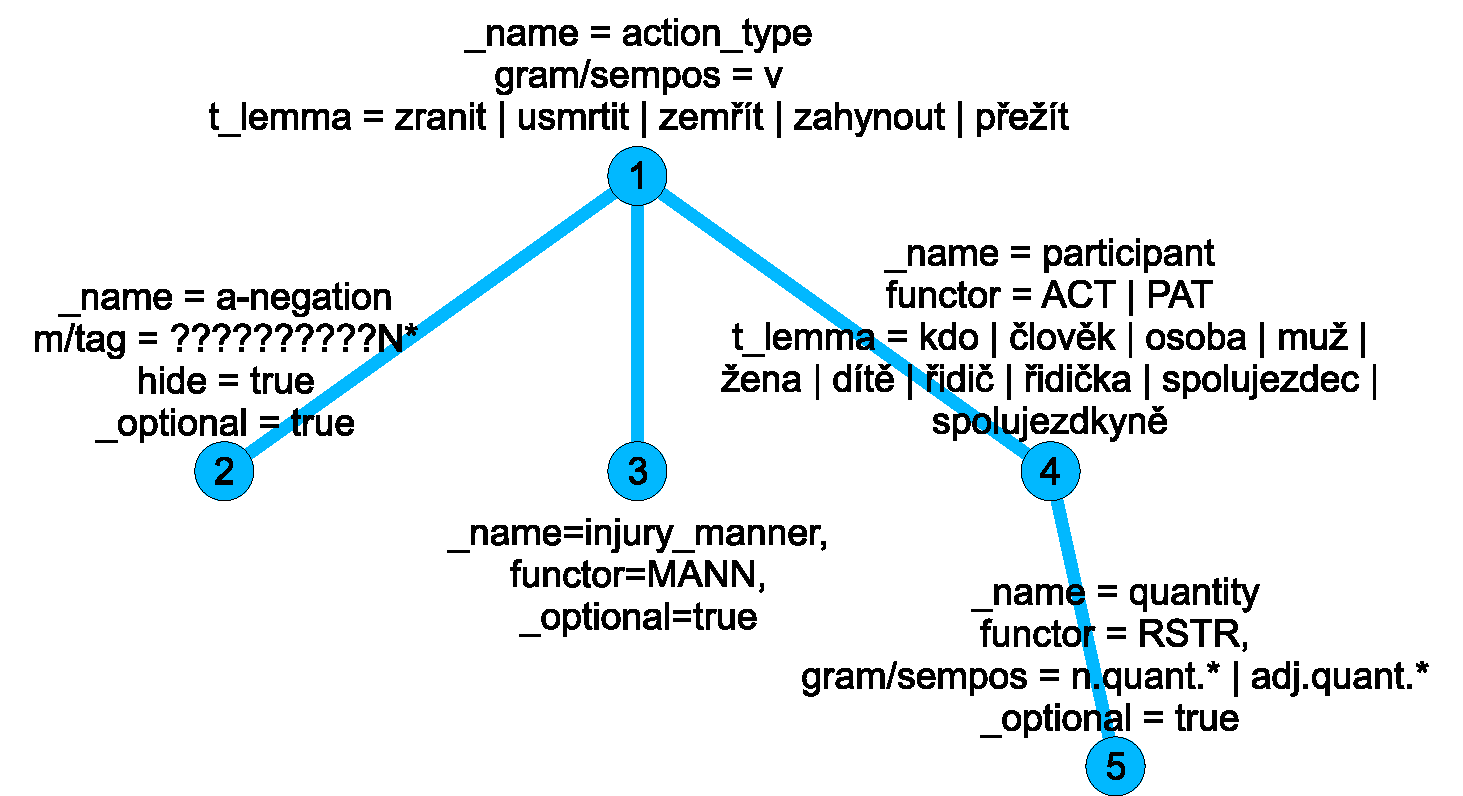
\includegraphics[width=0.9\hsize]{img/extract_patern}
%\end{center}
%\begin{itemize}
%	\item Tree patterns on \alert{shape} and \alert{nodes} (on node attributes).
%	\item Evaluation gives \alert{actual matches} of particular nodes.
%	\item \alert{Names} of nodes allow use of references.
%\end{itemize}
%\end{frame}
%
%
%
%
%\begin{frame}{Semantic interpretation of extraction rules}
%\begin{center}
%\includegraphics[width=\hsize]{img/DedVoj_semantic_interpretation}
%\end{center}
%\begin{itemize}
%	\item Determines how particular values of attributes are used.
%	\item Gives semantics to extraction rule.
%	\item Gives semantics to extracted data.
%\end{itemize}
%\end{frame}
%
%
%\begin{frame}{Accident attributes}
%\begin{columns}
%\column{.6\textwidth}
%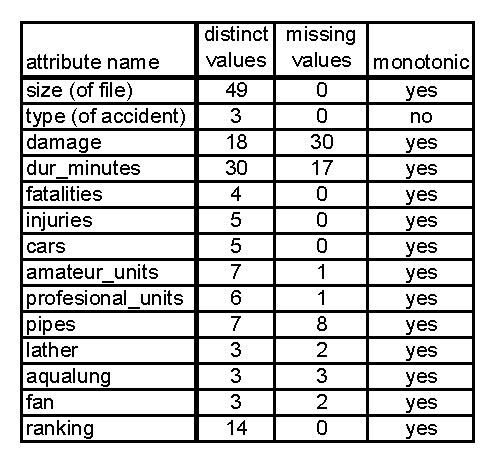
\includegraphics[height=0.75\vsize]{img/attributes_description}
%\column{.4\textwidth}
%\begin{itemize}
%	\item Information that we can/could extract from a report.
%\bigskip
%	\item Not everything is always mentioned.
%\end{itemize}
%\end{columns}
%\end{frame}
%
%
%
%\subsection{Fuzzy ILP}
%
%
%
%\begin{frame}{Classical ILP and Fuzzy ILP principles}
%\begin{itemize}
%	\item Learning examples $E=P\cup N$ (Positive and Negative)
%	\item Background knowledge $B$
%	\item ILP task -- to find hypothesis $H$ such that:
%\end{itemize}
%$$
%(\forall e\in P)(B\cup H\models e) \ \ \&\  \ (\forall n\in N)(B\cup H\not\models n).
%$$
%\vspace{0.5cm}
%\begin{itemize}
%	\item Fuzzy learning examples ${\mathcal E}:E\longrightarrow [0,1]$
%	\item Fuzzy background knowledge ${\mathcal B}:B\longrightarrow [0,1]$
%	\item Fuzzy ILP task -- to find hyp. ${\mathcal H}:H\longrightarrow [0,1]$ such that:
%\end{itemize}
%$$
%(\forall e_1,e_2\in E)(\forall {\mathcal M})({\mathcal M}\models_f {\mathcal B}\cup {\mathcal H}) \ :\ 
%{\mathcal E}(e_1)>{\mathcal E}(e_2)\Rightarrow \left\|e_1\right\|_{{\mathcal M}}\ge \left\|e_2\right\|_{{\mathcal M}}
%$$
%\end{frame}
%
%\begin{frame}{Generalized Annotated Programs}
%\begin{itemize}
%	\item Fuzzy ILP is equivalent to Induction of Generalized Annotated Programs\footnote{See in S. Krajci, R. Lencses and P. Vojtas: ``A comparison of fuzzy and annotated logic programming'', Fuzzy Sets and Systems, vol.144, pp.173�192, 2004.}
%	\item For implementation we use GAP or strictly speaking: \emph{Definite Logic Programs with monotonicity axioms} (also equivalent)
%	\item Basic paradigm: deal with \alert{values} as with \alert{degrees}.
%		\begin{itemize}
%			\item We don't have to normalize values, they order is enough.			
%		\end{itemize}
%	\medskip
%	\item For example with monotonicity axioms we can use rule:
%\centerline{\texttt{serious(A, 4)} $\leftarrow$ \texttt{fatalities(A, 10).}}
%	and form the fact \texttt{fatalities(id\_123, 1000)} deduce
%\centerline{\texttt{serious\_alt(id\_123, 4).}}
%\end{itemize}
%\end{frame}
%
%
%
%\section{Our Experiment}
%\subsection{Experiment Description}
%
%\begin{frame}{Accident attributes}
%\begin{columns}
%\column{.6\textwidth}
%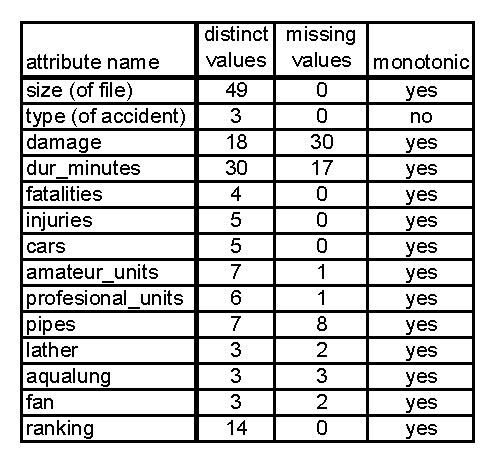
\includegraphics[height=0.75\vsize]{img/attributes_description}
%\column{.4\textwidth}
%\begin{itemize}
%	\item Almost all attributes are \alert{numeric}.
%		\begin{itemize}
%			\item So \alert{monotonic}
%			\item This will be used for ``fuzzyfication''
%		\end{itemize}
%\bigskip
%	\item Artificial target attribute \alert{seriousness ranking}.
%\end{itemize}
%\end{columns}
%\end{frame}
%
%
%\begin{frame}{Histogram of the seriousness ranking attribute}
%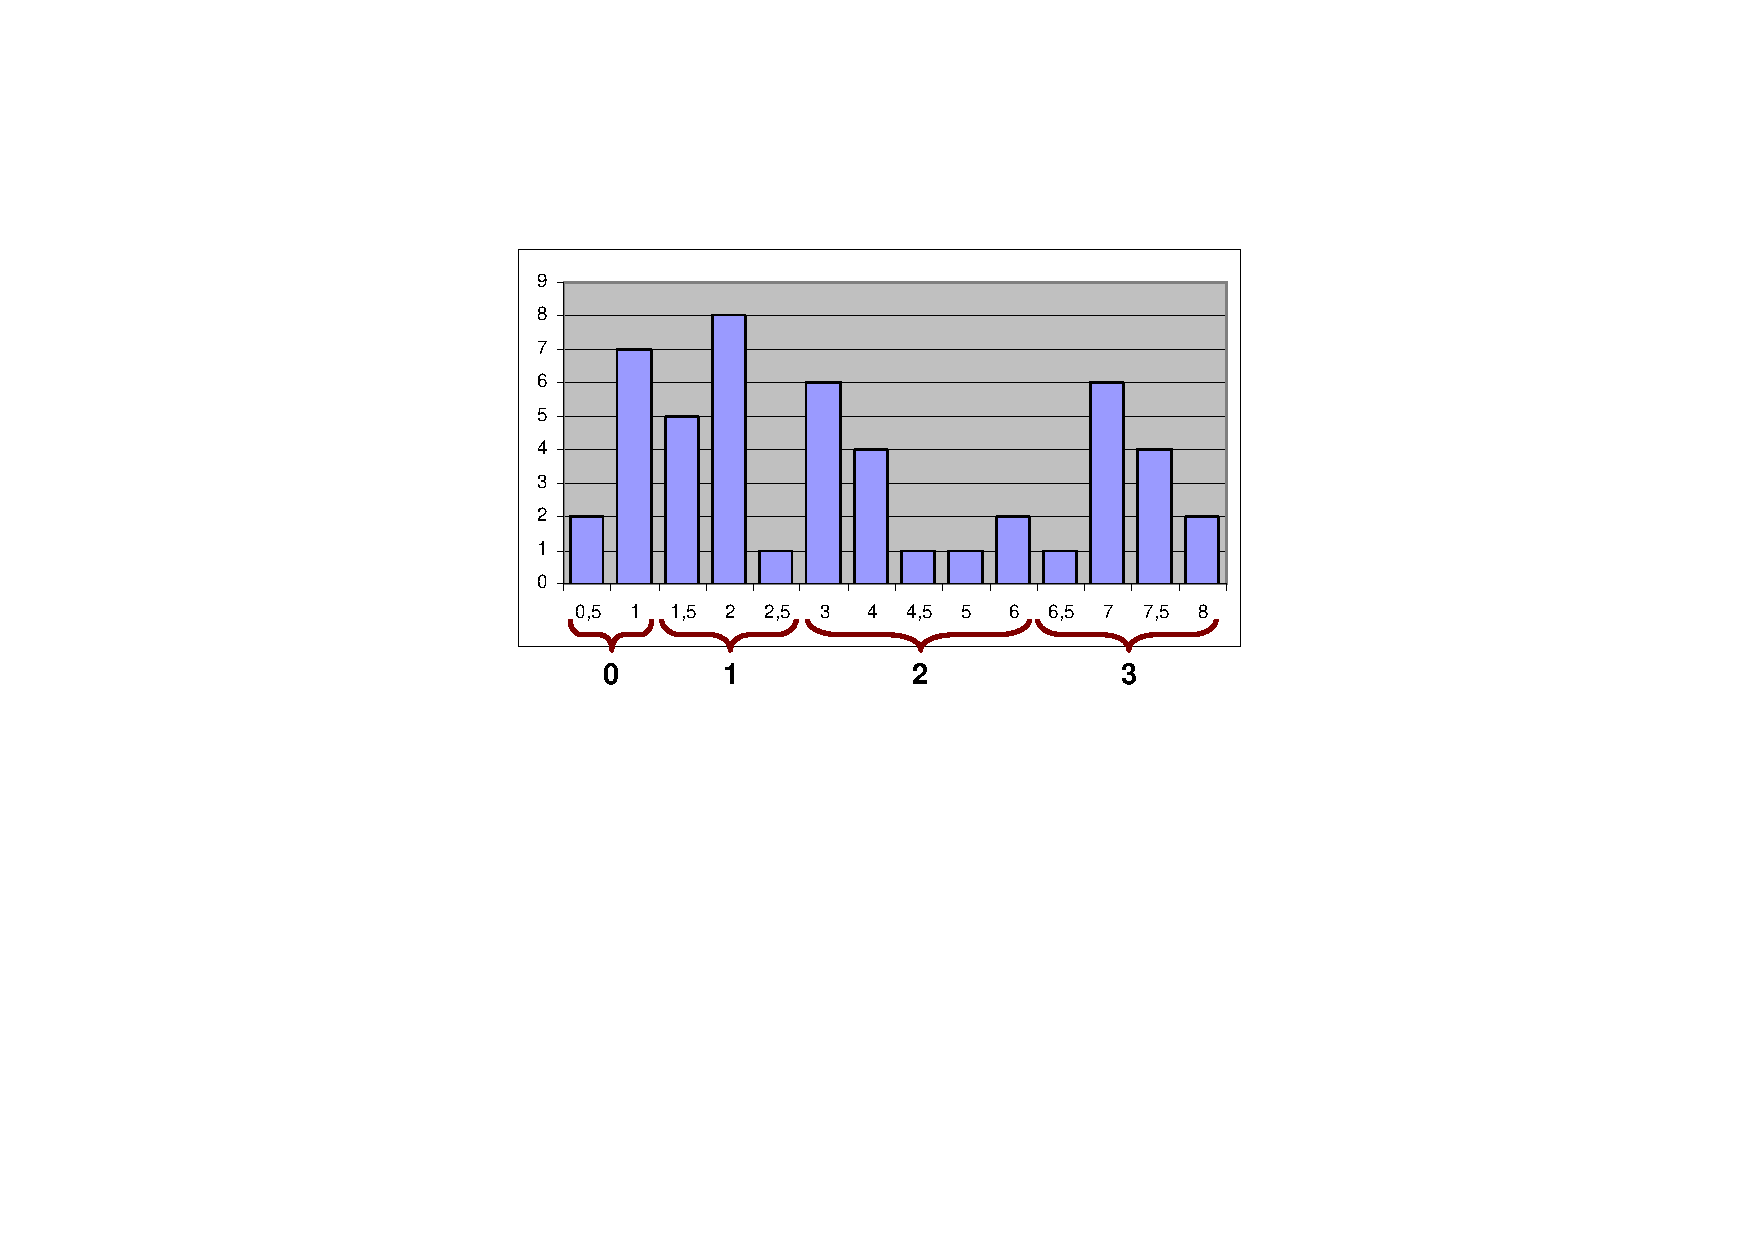
\includegraphics[width=0.9\hsize]{img/ranking_histogram}
%\begin{itemize}
%	\item 14 different values, range 0.5 -- 8
%	\item Divided into four approximately \alert{equipotent groups}.
%\end{itemize}
%\end{frame}
%
%
%
%\section{Fuzzy ILP / GAP Implementation}
%\subsection{Monotonization}
%
%
%
%\begin{frame}{Essential difference between learning examples}
%\begin{columns}
%\column{.6\textwidth}
%\setbeamercolor{block title}{bg=BrickRed}
%\begin{block}{Crisp learning examples}
%\centerline{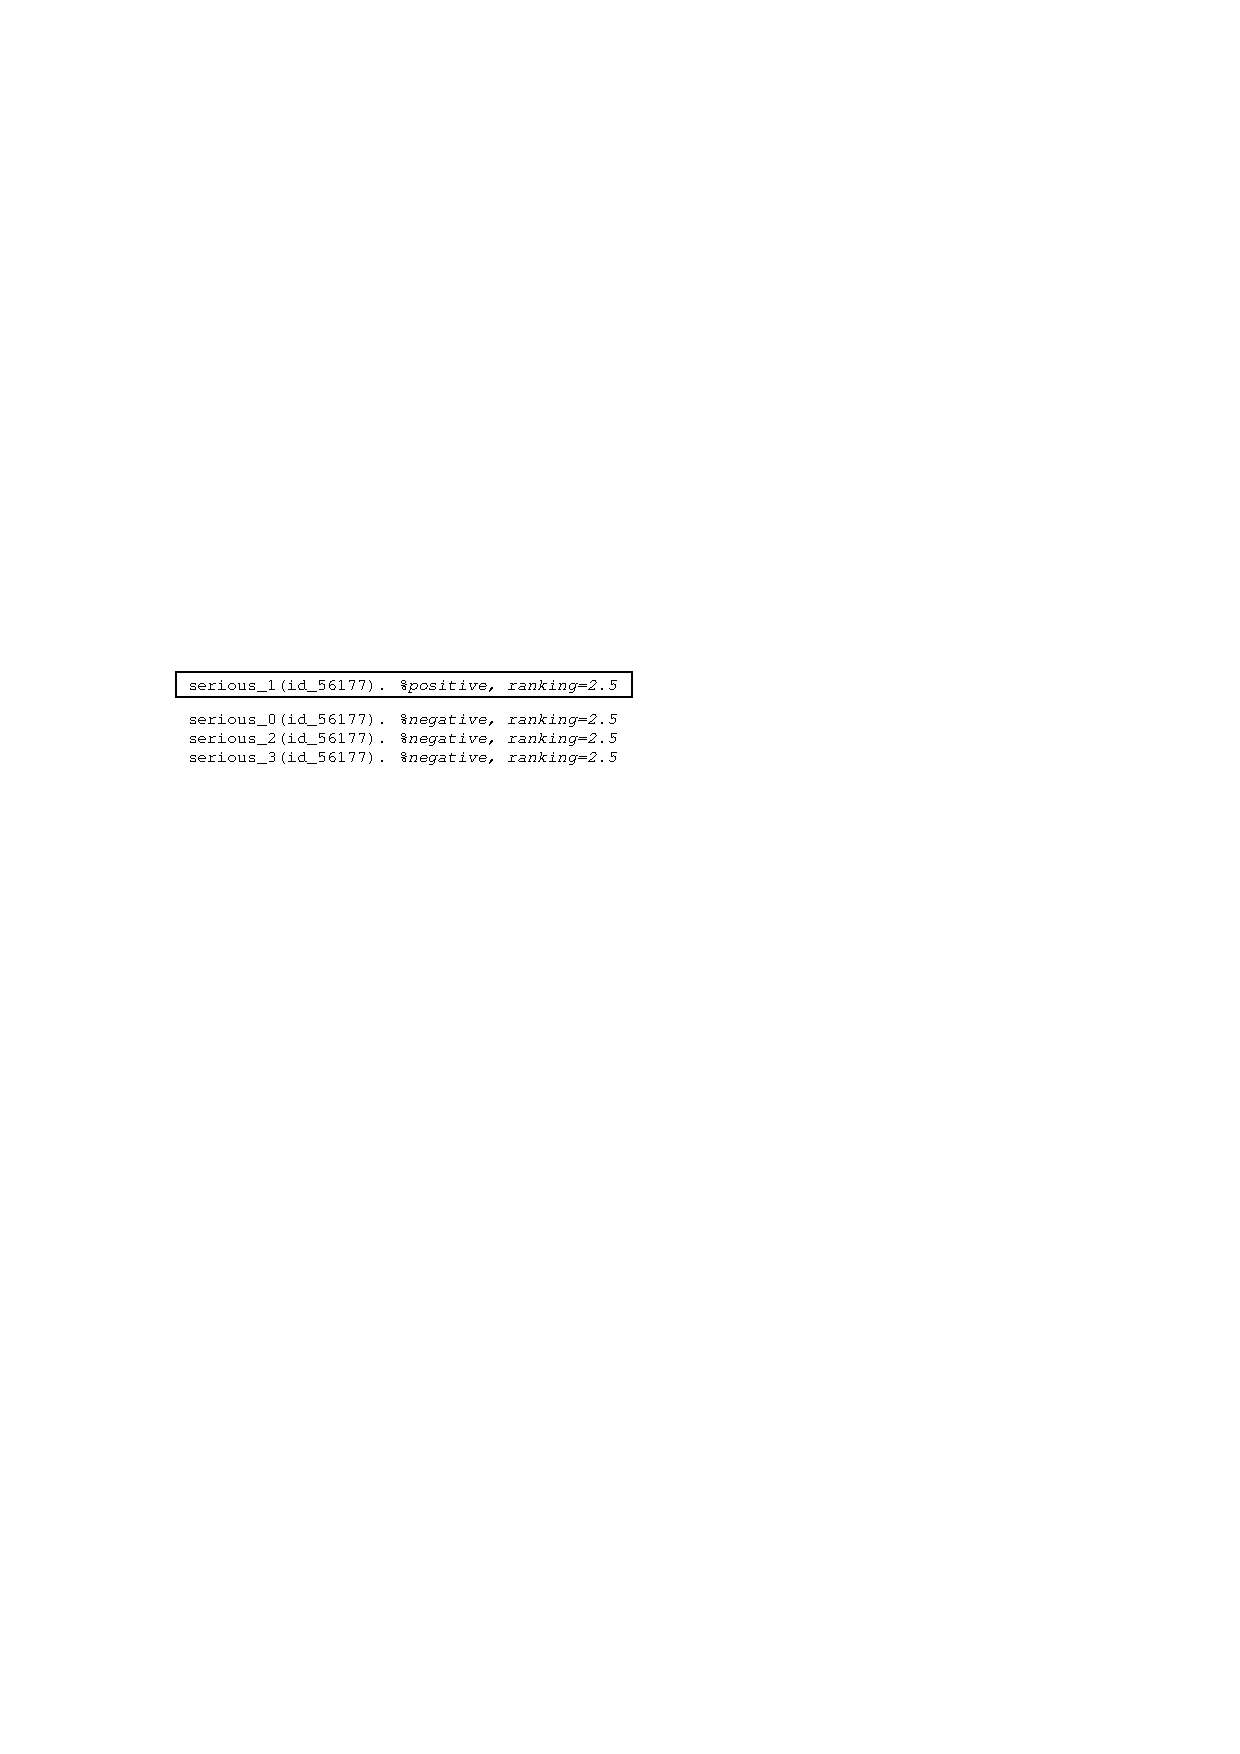
\includegraphics[width=\hsize]{img/examples_nonmonot}}
%\end{block}
%\bigskip
%\setbeamercolor{block title}{bg=OliveGreen}
%\begin{block}{Monotonized learning examples}
%\centerline{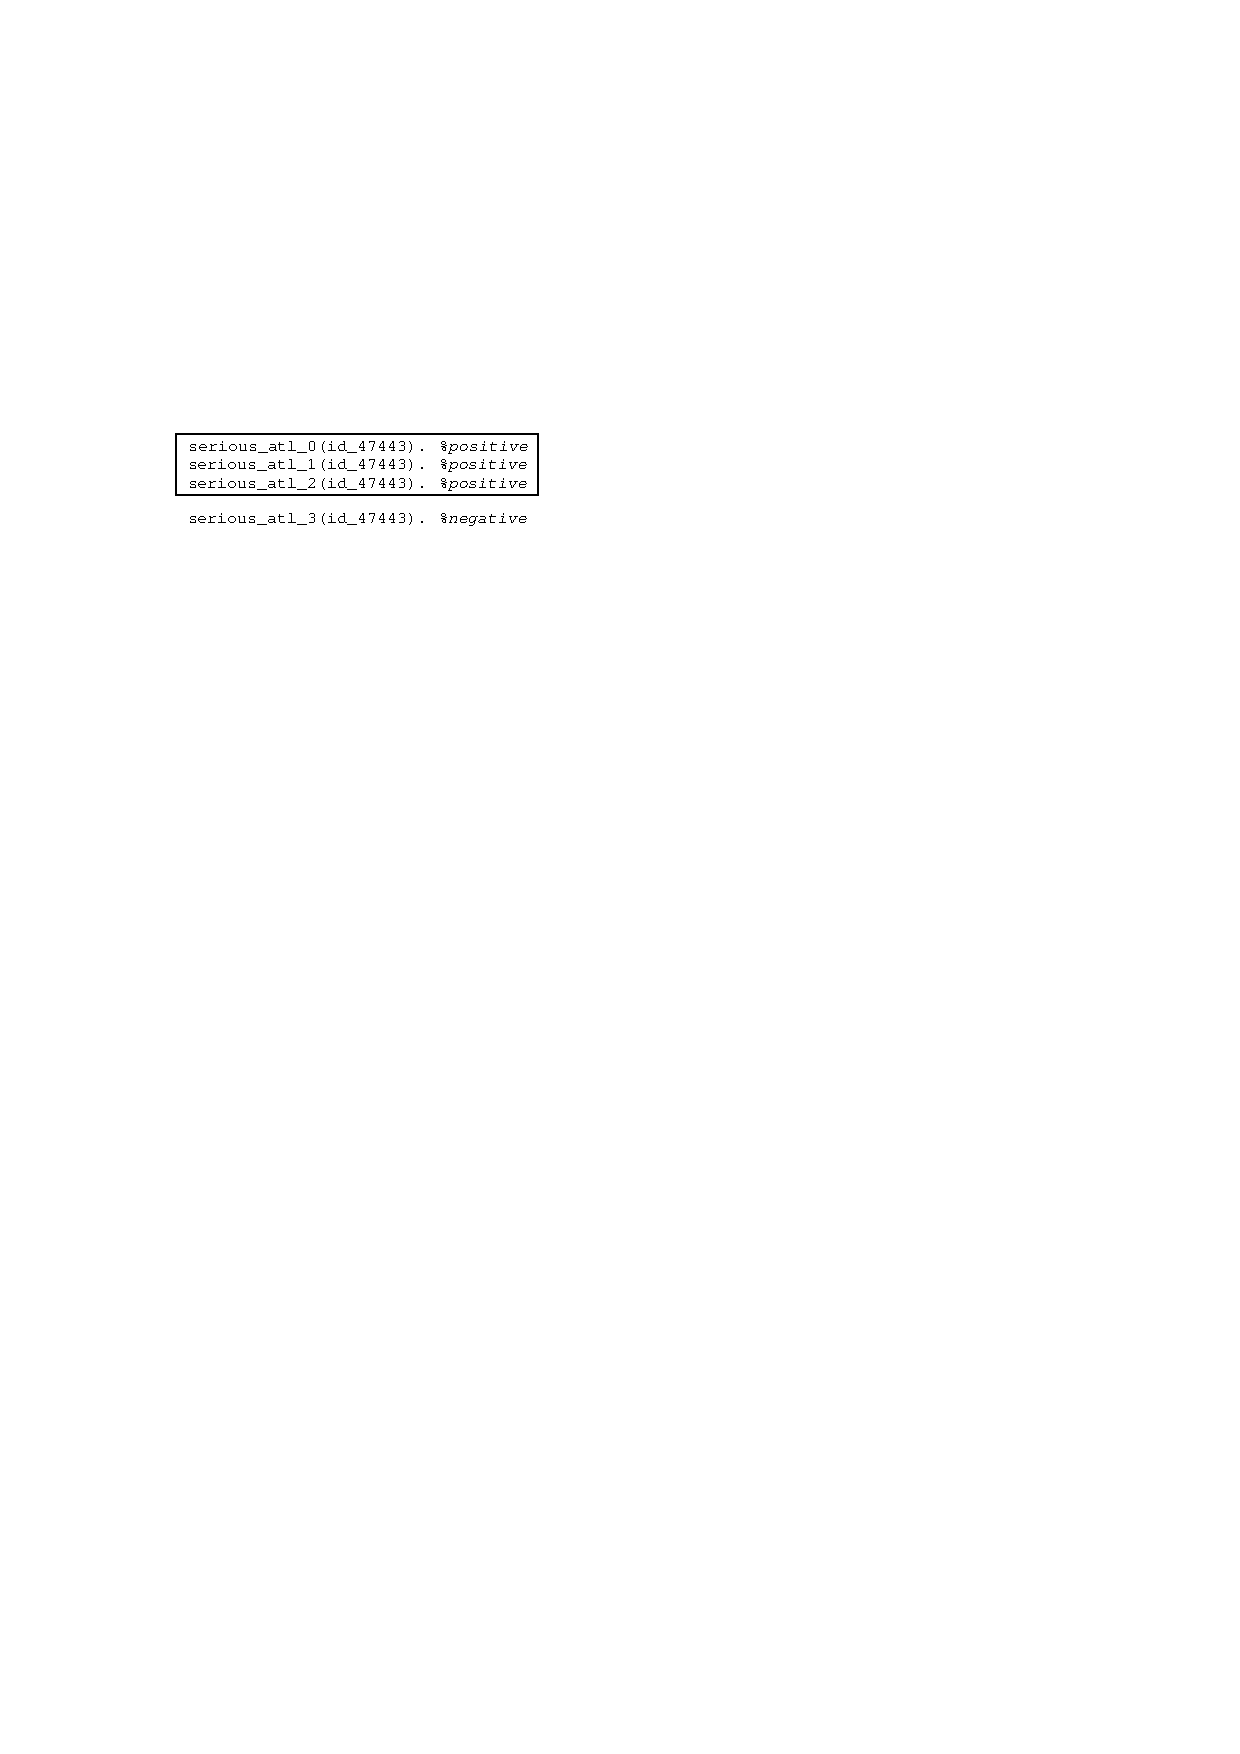
\includegraphics[width=\hsize]{img/examples_monot}}
%\end{block}
%\column{.4\textwidth}
%For one evidence (occurrence):
%	\bigskip
%\begin{itemize}
%	\item Crisp:\\
%	Always \alert{one} positive and \alert{three} negative learning examples
%	\bigskip
%	\item Monotonized:\\
%	\alert{Up to the observed degree} positive,\\the rest negative.
%\end{itemize}
%\end{columns}
%\end{frame}
%
%
%\begin{frame}{Monotonization of attributes}
%\definecolor{MyBrown}{rgb}{0.5,0.5,0}
%\setbeamercolor{block title}{bg=MyBrown}
%\begin{block}{damage\_atl $\leftarrow$ damage}
%\centerline{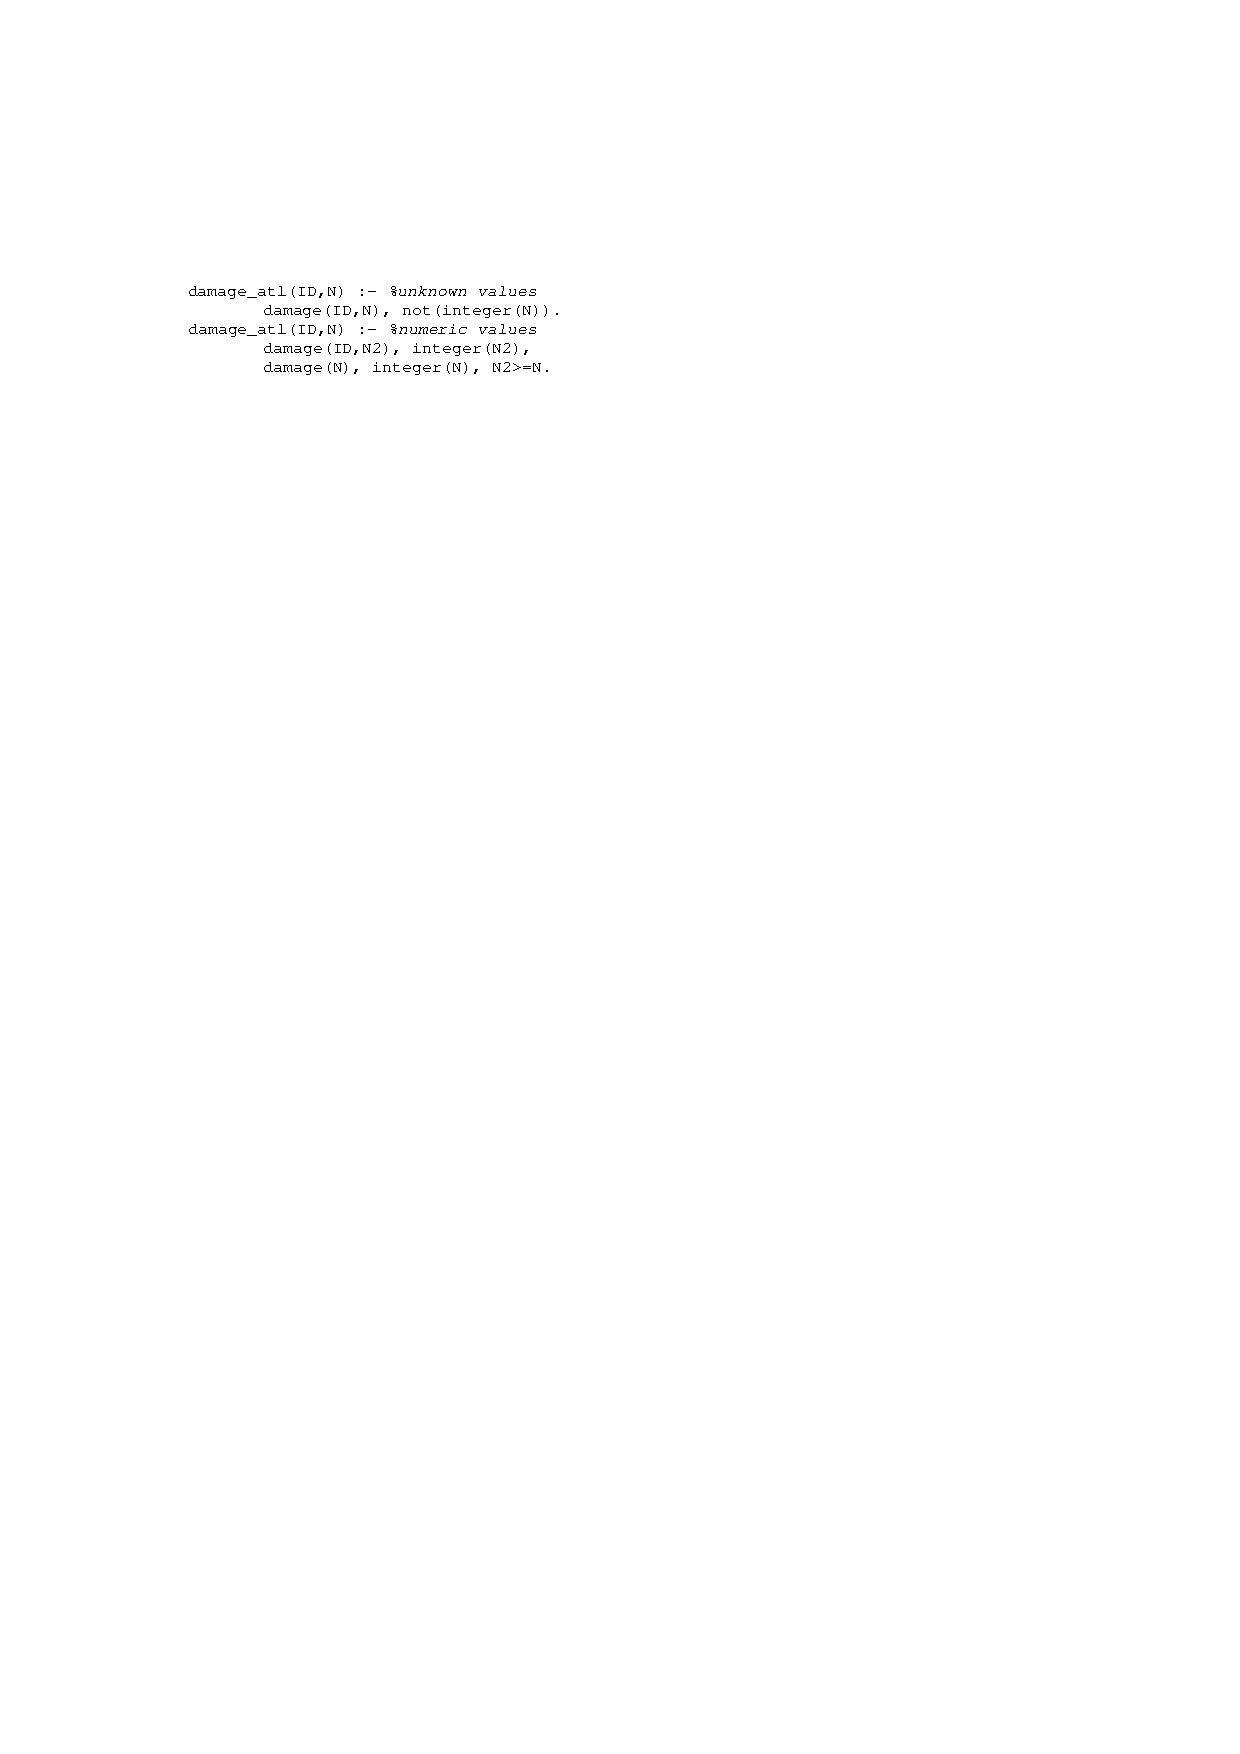
\includegraphics[width=0.73\hsize]{img/attribute_monotonisation}}
%\end{block}
%\bigskip
%\begin{itemize}
%	\item We infer all lower values as sufficient.
%	\item Treatment of unknown values.
%	\item Negation as failure.
%\end{itemize}
%\end{frame}
%
%\section{Evaluation and Conclusion}
%\subsection{Learning Results}
%
%\begin{frame}[plain]%{Crisp \& monotonized hypothesis}
%\begin{columns}
%\column{.67\textwidth}
%\centerline{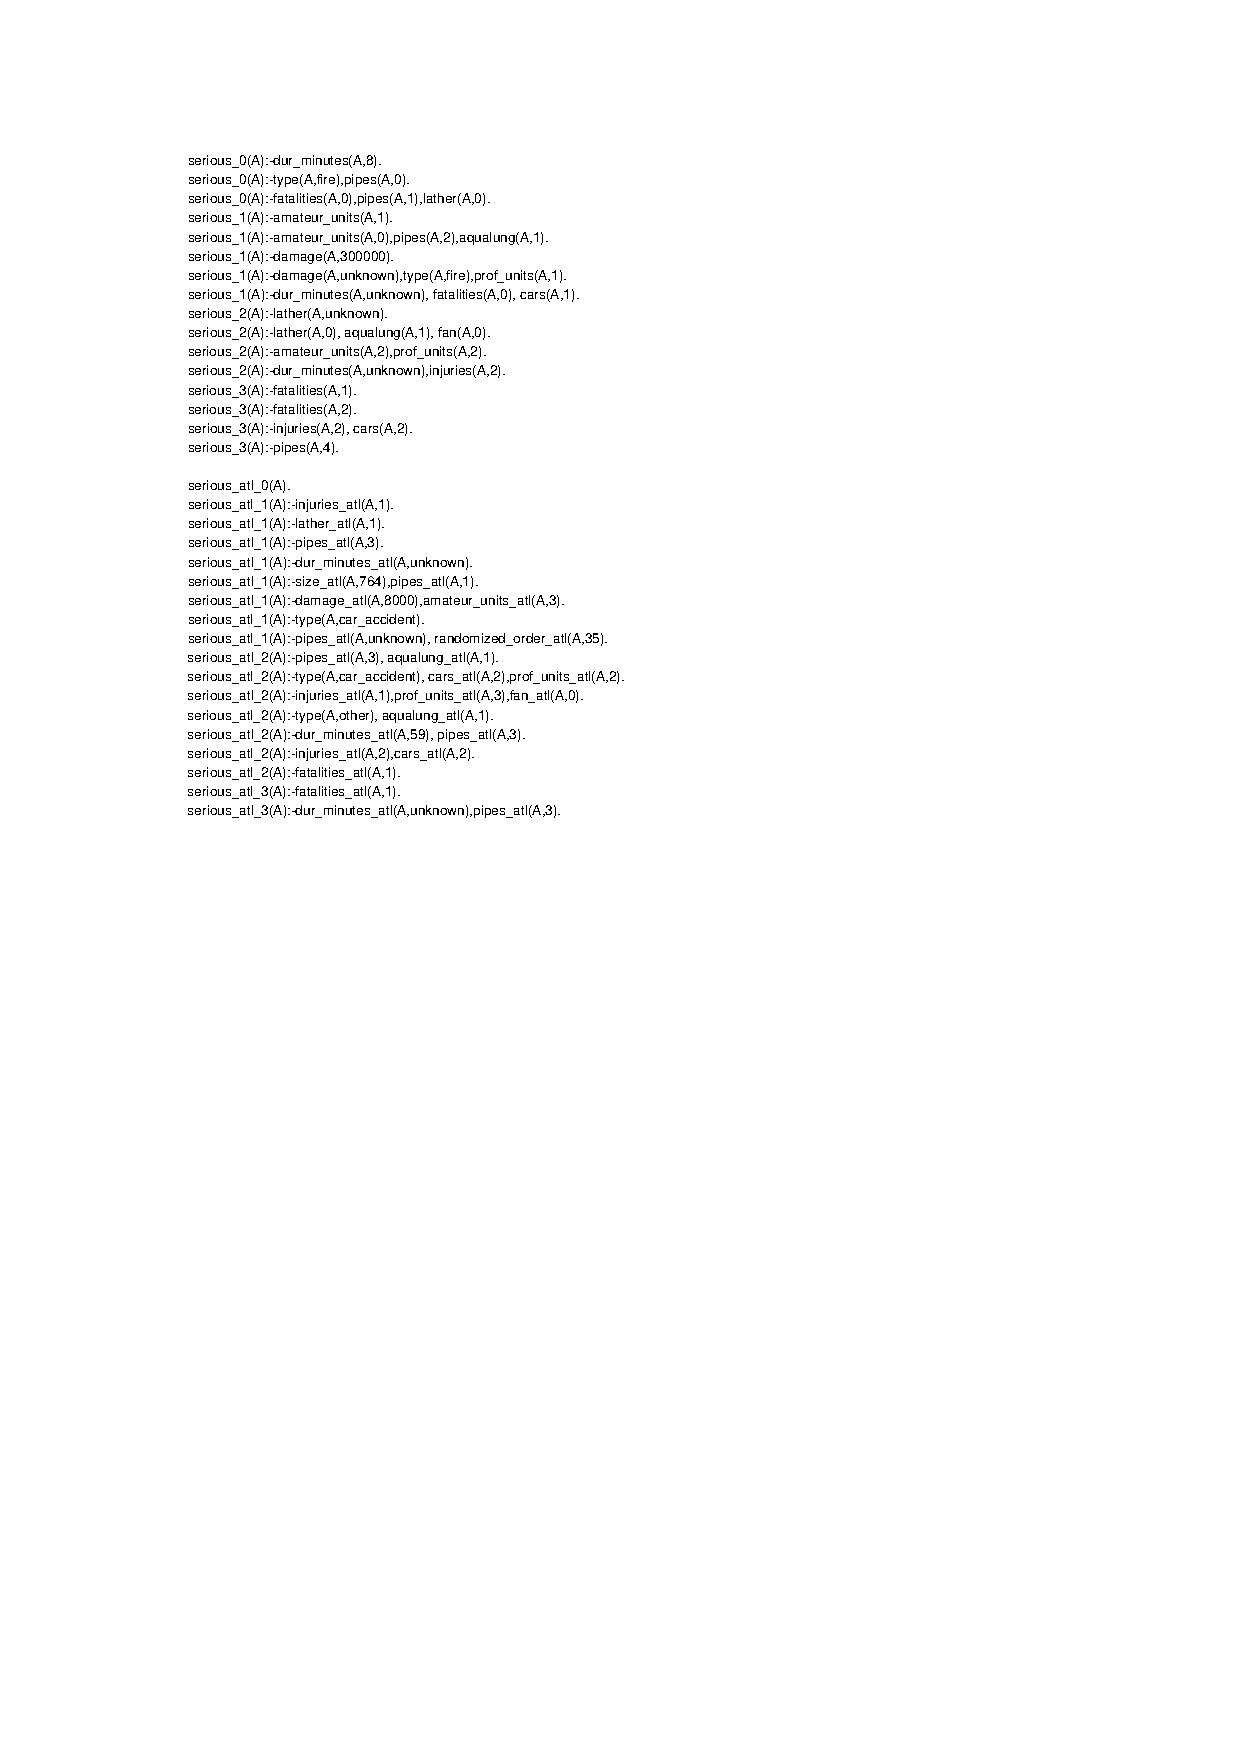
\includegraphics[height=1.1\vsize,width=\hsize]{img/rules}}
%\column{.33\textwidth}
%\begin{itemize}
%	\item Crisp hypothesis
%\vspace{3cm}
%	\item Monotonized hypothesis	
%	\begin{itemize}
%		\item Monotonicity axioms
%		\item Monotonized learning examples
%	\end{itemize}
%\end{itemize}
%\vspace{2cm}
%\end{columns}
%\end{frame}
%
%\subsection{Evaluation}
%
%\begin{frame}{Evaluation and Comparison of Results}
%\centerline{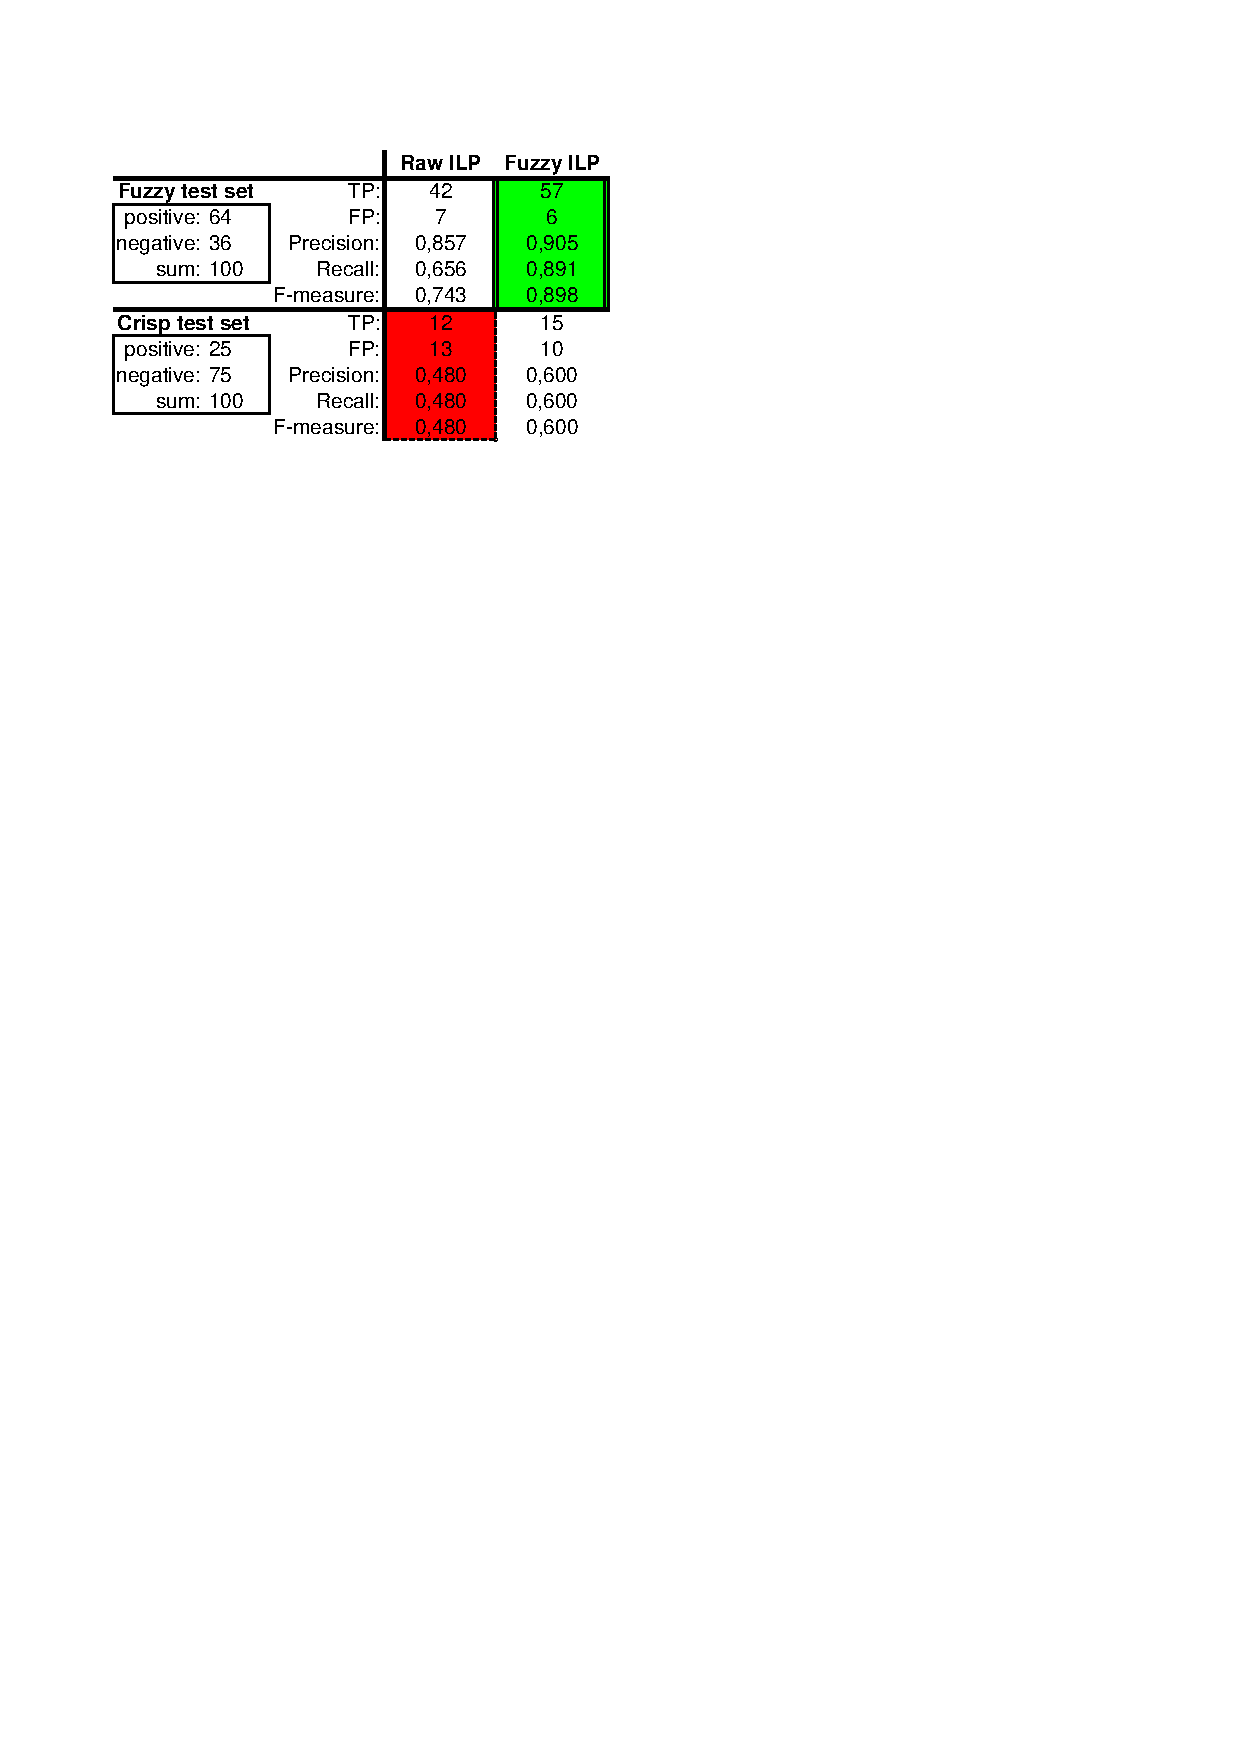
\includegraphics[width=0.75\hsize]{img/Evaluation}}
%\bigskip
%\begin{itemize}
%	\item Rules evaluated on both testing sets.
%		\begin{itemize}
%			\item By use of conversion predicates (next slide)
%		\end{itemize}
%	\item Monotonized rules \alert{better in both cases}.
%\end{itemize}
%\end{frame}
%
%
%
%\begin{frame}{Conversion of Results}
%\setbeamercolor{block title}{bg=BrickRed}
%\begin{block}{crisp $\leftarrow$ monotone}
%\centerline{
\includegraphics[width=.8\hsize]{img/monot2nomon}}
%\end{block}
%\bigskip
%\setbeamercolor{block title}{bg=OliveGreen}
%\begin{block}{monotone $\leftarrow$ crisp}
%\centerline{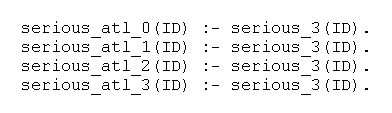
\includegraphics[width=.8\hsize]{img/nomon2monot}}
%\end{block}
%\end{frame}
%
%\subsection{Conclusion}
%
%\begin{frame}{Conclusion}
%\begin{itemize}
%	\item We used Fuzzy/GAP ILP in an \alert{experiment}\\ closely connect with WIE.
%	\item Showed basic \alert{principles and implementation}\\ of Fuzzy/GAP ILP.
%	\item Compared results of Fuzzy/GAP ILP and Classical ILP.
%	\item Observed much better results in the Fuzzy case.
%	\bigskip
%	\item Future work:
%	\begin{itemize}
%		\item Improvement of the extraction method
%		\item Other languages, other domains 
%\medskip
%		\item Finer ``approximatization'' of target attribute (not only ``four degrees'').
%%		\item Learn the target attribute directly.
%	\end{itemize}
%\end{itemize}
%\end{frame}
%
%
%\end{document}
%
%
